%%%%%%%%%%%%%%%%%%%%%%%%%%%%%%%%%%%%%%%%%%%%%%%%%%%%%%%%%%%%%%%%%
% Qualificacao de Doutorado / Dept Fisica, CFM, UFSC            %
% Eduardo@UFSC - 2015                                           %
%%%%%%%%%%%%%%%%%%%%%%%%%%%%%%%%%%%%%%%%%%%%%%%%%%%%%%%%%%%%%%%%%


%:::::::::::::::::::::::::::::::::::::::::::::::::::::::::::::::%
%                                                               %
%                          Capítulo 6                           %
%                                                               %
%:::::::::::::::::::::::::::::::::::::::::::::::::::::::::::::::%

%***************************************************************%
%                                                               %
%                      Conversão tauV - Gas                     %
%                                                               %
%***************************************************************%

\chapter{Estimando frações de gás}
\label{sec:gasfrac}

Durante a pesquisa que nos levou a escrever o artigo que está no Apêndice \ref{apendice:GDetal2014b}
encontramos uma relação interessante que serviu de pontapé inicial para explorarmos a conversão de
poeira em gás. Nesse capítulo vamos comentar brevemente sobre nosso progresso e discutir quais os
desafios enfrentados até agora e aqueles que estão por vir nas próximas estapas de nosso projeto.

\section{Um modelo simples de evolução química}
\label{sec:gasfrac:closedbox}

Em um modelo simples de evolução química assume-se:
\begin{itemize}
	\setlength\itemsep{0.2cm}
  	\item não existir nem {\em inflow} nem {\em outflow} de gás na galáxia (isolada em um sistema
fechado sem entrada nem saída de gás);
  	\item seu gás inicial não possui metais (metalicidade inicial do sistema é zero);
  	\item {\em Instantaneous Recycling Approximation}: todas as estrelas com mais de 1
$M_\odot$ evoluem e morrem imediatamente e todas as estrelas com massa menor que 1 $M_\odot$ vivem
eternamente;
	\item a IMF é constante no tempo;
	\item o gás está sempre homogeneamente misturado.
\end{itemize}

Com estas simplificações, podemos escrever a metalicidade do gás como:
\begin{equation}
	Z_{\mathrm{gas}}\ =\ y \ln \left(\frac{1}{f_{\mathrm{gas}}}\right),
	\label{eq:Zgas_closedbox}
\end{equation}
\noindent onde $y$ é o {\em yield} estelar (também conhecido como {\em true yield}), portanto a
fração de gás no modelo simples de evolução química ({\em closed-box model}) determina a
metalicidade do gás. Antes de prosseguir, vamos definir fração de gás como:
\begin{equation}
	f_{\mathrm{gas}}\ =\ \frac{M_{\mathrm{gas}}}{M_\star + M_{\mathrm{gas}}}\ =\ \frac{1}{1 +
	\left(\frac{M_\star}{M_{\mathrm{gas}}}\right)}\ \equiv\ \frac{1}{1 +
	\left(\frac{\mu_\star}{\SigmaGas}\right)}
	\label{eq:fgas}
\end{equation}
\noindent onde $M_{\mathrm{gas}}$ é a massa total na forma de gás e $M_\star$ é a massa total em
estrelas e $\mu_\star$ e $\SigmaGas$ são as densidades superficiais de massa estelar e de massa de
gás.

A relação da qual comentamos no preâmbulo deste capítulo pode ser vista na Fig.
\ref{fig:dust2stars}. A razão entre o coeficiente de extinção (em magnitude) e a densidade
superficial de massa estelar ($A_V / \mu_\star$) parece relacionar de maneira interessante com a
metalicidade média das populações estelares. Dado que poeira ($A_V$) pode ser tomada como indicador
de gás, essa relação empírica sugere que Z decresce à medida que cresce a proporção gás/estrelas, o
que é condizente com a ideia de que ao passar do tempo, o processo de formação estelar vai
enriquecendo quimicamente o gás (ao passo que o consome), fazendo com que as novas gerações de
estrelas tenham maior metalicidade.
 
\begin{figure}
	\centering
	%\resizebox{0.7\textwidth}{!}{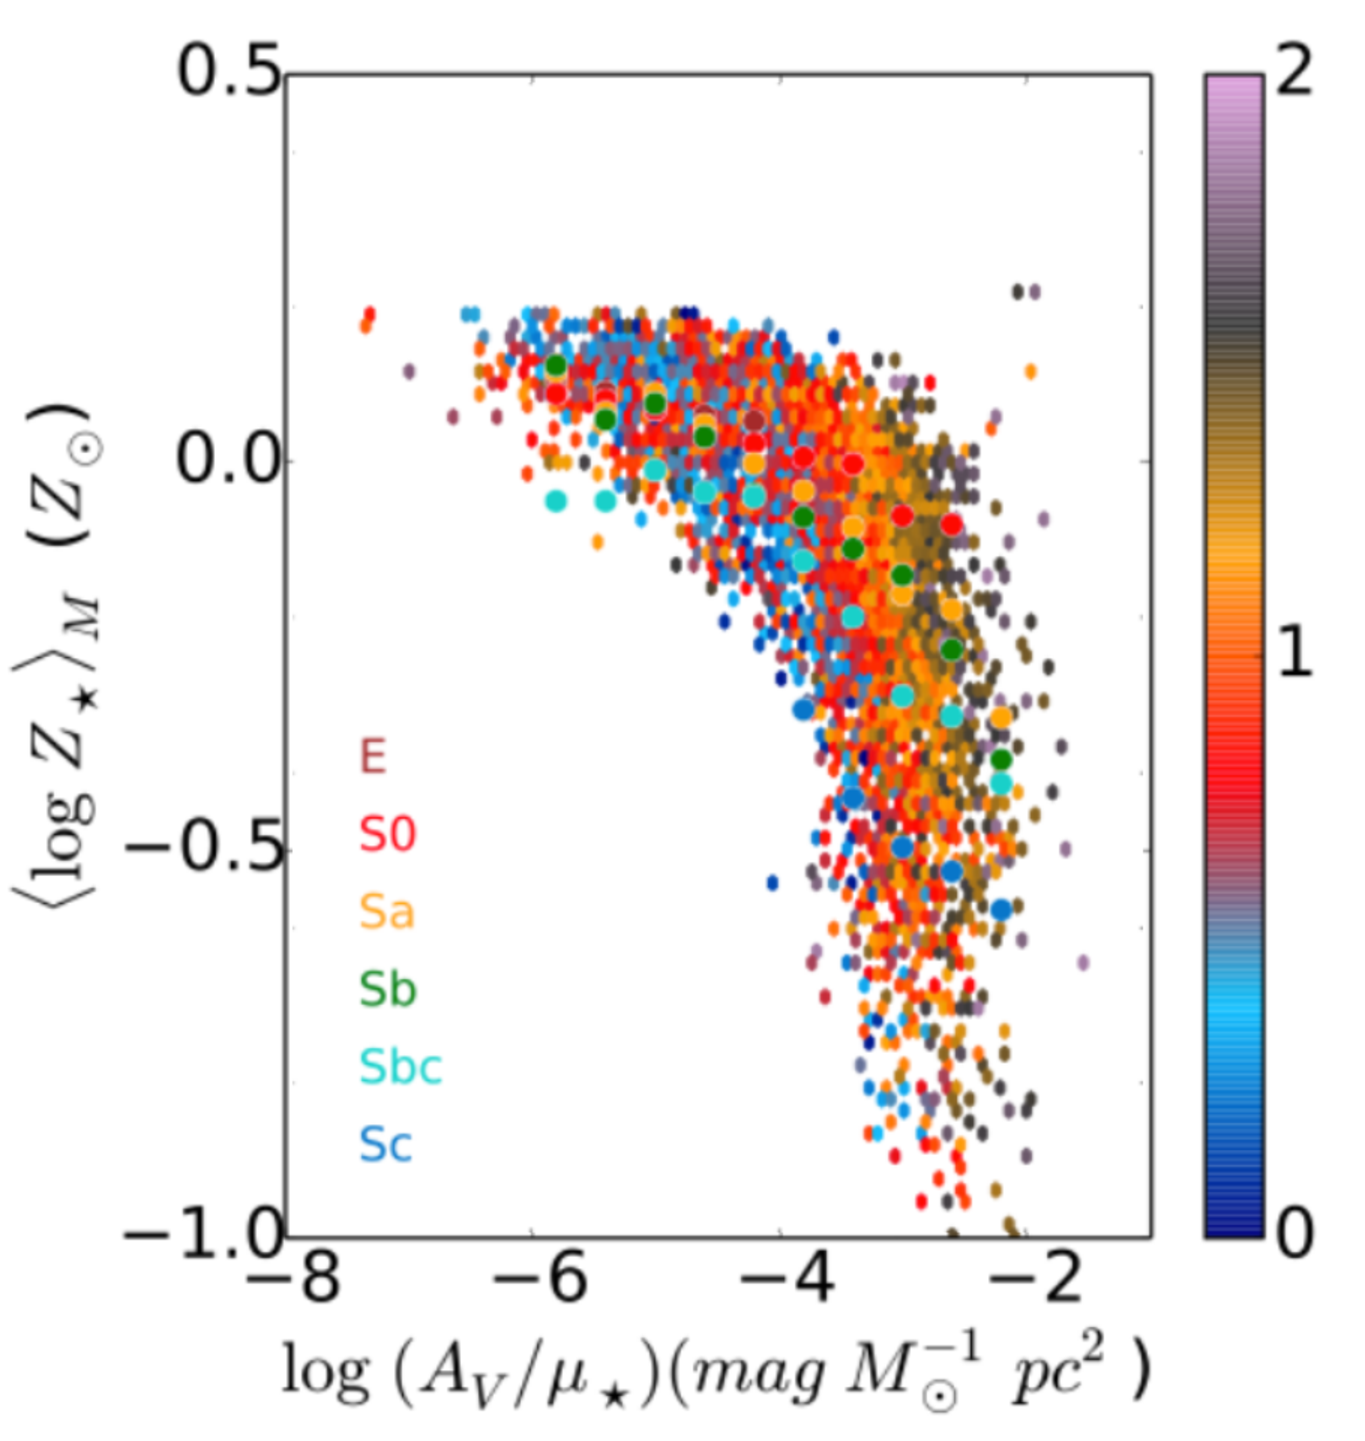
\includegraphics{figuras/dust2stars.pdf}}
	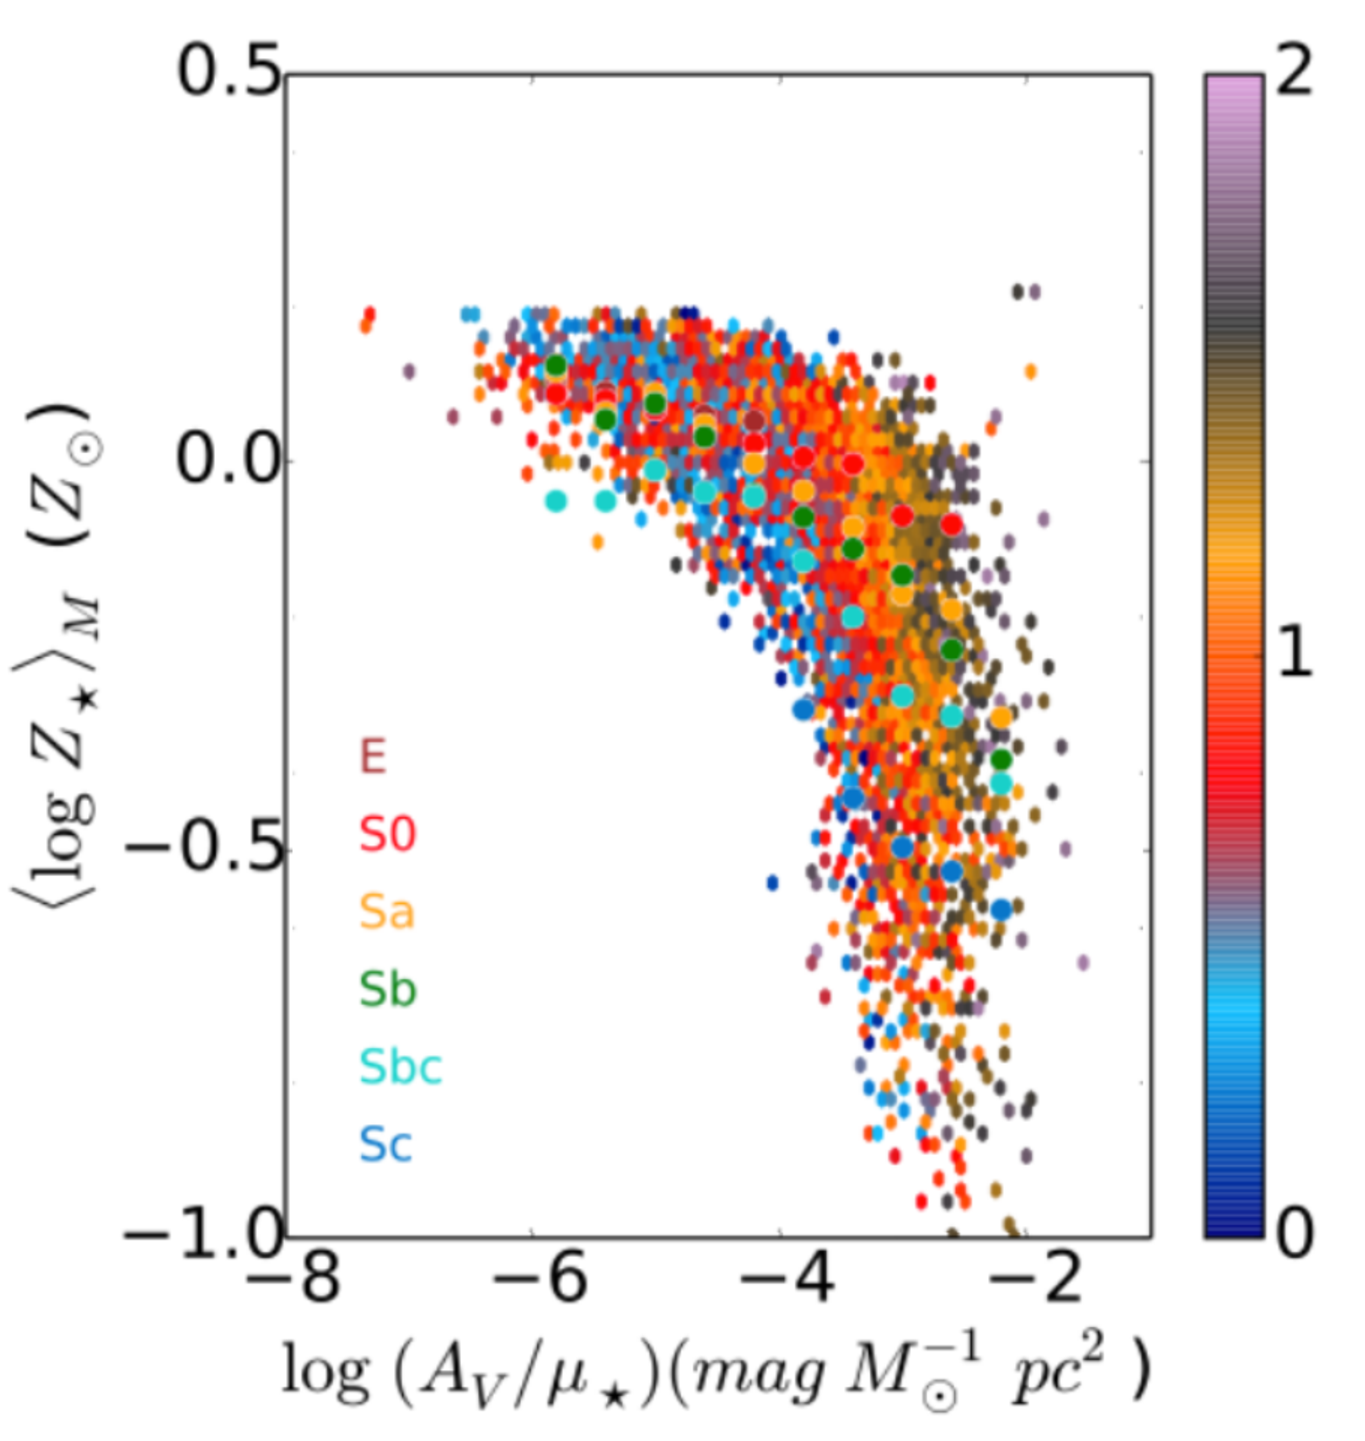
\includegraphics[height = 8cm, width = 9.5cm]{figuras/dust2stars.pdf}
	\caption[$A_V / \mu_\star$ vs. \meanM{\log Z_\stars}]
	{Relação entre metalicidade média das populações estelares e a razão entre o coeficiente de
extinção (em magnitude) e a densidade superficial de massa estelar. Os pontos são aproximadamente
6000 bins radiais de 300 galáxias (de 0 a 2 HLR divididos em 20 bins por galáxia) e estão
classificados em cores por tipo morfológico.}
	\label{fig:dust2stars}
\end{figure} 

Invertendo \eqref{eq:Zgas_closedbox} podemos definir o {\em yield} efetivo ($y_{eff}$), ou seja,
aquele que um sistema teria caso se comportasse como dito modelo ao longo de toda a linha do tempo.
Essa primeira equação foi derivada explicitamente pela primeira vez por \citet{Searle.Sargent.1972a}
ao estudar duas regiões \Hii gigantes, ditas ``isoladas''. \citet{Garnett.2002a}, assumindo um {\em
true yield} constante, calcula $y_{eff}$ para 31 galáxias espirais e 13 galáxias irregulares,
encontrando valores distintos entre elas, o que o leva a concluir que o fluxo de gás ({\em outflow}
e {\em inflow}) nestes sistemas são ambos processos muito importantes para a evolução química de uma
galáxia. \citet{Tremonti.etal.2004a} calculam o $y_{eff}$ para $\sim 55000$ galáxias {\em
star-forming} do \SDSS. Ao adicionar outras medidas verifica que este valor varia em uma escala de
$\sim 10$ vezes, o que falha com a assunção de um {\em yield} constante. 

\section{Relação de Kennicutt-Schmidt e a pseudo-KS}
\label{sec:gasfrac:KS}

\begin{figure}
	\centering
	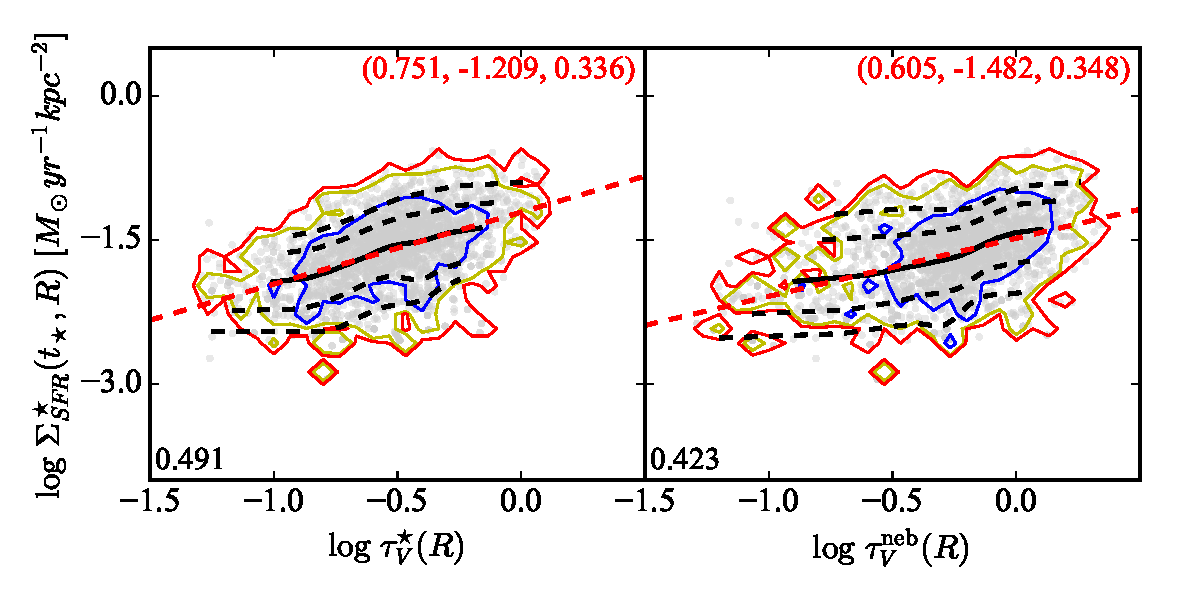
\includegraphics[width=0.8\textwidth]{figuras/pseudoKS.pdf}
	\caption[Relação pseudo-KS]
	{Relação entre a densidade superficial da taxa de formação estelar e o coeficiente de extinção
proveniente da síntese ($\tauVS$ - {\em painel esquerdo}) e do decremento de Balmer ($\tauVN$ -
{\em painel direito}). Em ambos painéis as linhas pretas marcam a mediana (linha contínua) e os 5,
16, 64 e 95 percentis (linhas tracejadas). A linha tracejada em vermelho marca o ajuste linear da
mediana e os valores marcam o coeficiente de correlação de Spearmann (canto inferior esquerdo) e a
inclinação, valor de y no qual há a interceptação do eixo x e o valor do desvio médio quadrático da
distribuição em torno do ajuste (canto superior direito).}
	\label{fig:pseudoKS}
\end{figure}

Como explicado na Sec. \ref{sec:intro:galaxias}, a quantidade de gás de uma galáxia e a taxa de
formação estelar estão relacionadas através de uma lei de potências (KS). A relação entre poeira e
formação estelar é um resultado de indireto desta lei já que vemos que existe a ligação entre poeira
e gás e que ela possui dependência com a metalicidade nebular principalmente \citep[][e suas
referências]{Magdis.etal.2011a, Leroy.etal.2011a, Santini.etal.2014a}. Pensando nisso, vamos estudar
a relação entre poeira e formação estelar (aqui chamada de pseudo-KS - $pKS$), que pode ser vista na
Fig. \ref{fig:pseudoKS}. No painel esquerdo usamos $\tauVS$ como variável representante da poeira e
no direito, $\tauVN$. O espalhamento nesta figura nos mostra que podemos explorar os resíduos em
torno desse ajuste, mas é bastante claro que existe uma relação. Vamos agora estudar a natureza
do resíduo em torno do ajuste da mediana da distribuição com $\tauVS$ (linha tracejada vermelha na
Fig. \ref{fig:pseudoKS}), através da equação:
\begin{eqnarray}
	\log\ \SigmaSFR(\tauVS)\ &=&\ 0.751 \log\ \tauVS - 1.209 \\
	\label{eq:pKS_1stadj}
	\Delta(pKS)\ &=&\ \log\ \SigmaSFR - (0.751 \log\ \tauVS - 1.209).
	\label{eq:DeltapKS}
\end{eqnarray}

\subsection{Resíduos da pseudo-KS}
\label{sec:gasfrac:KS:resid}

O resíduo vem de \eqref{eq:DeltapKS}. Na Fig. \ref{fig:deltapKS} vemos com detalhe o resíduo frente
a diversas propriedades. De todas elas as maiores correlações com $\Delta(pKS)$ são com a densidade
superficial de massa estelar, o raio, a metalicidade nebular e a fração em luz das populações
jovens. Apesar da notável participação da metalicidade nebular no espalhamento da relação $pKS$, ela
possui intervalo pequeno de variação (90\% dos pontos ficam no intervalo entre -0.4 e -0.11
$Z_\odot$), além do resíduo ir para o lado contrário que imaginaríamos assumindo que, para um
$\tauVS$ fixo, com o aumento da metalicidade $\SigmaGas$ (e consequentemente, $\SigmaSFR$) deveria
diminuir (causando um resíduo na direção contrária). A densidade superficial de massa estelar parece
ser a principal causadora do espalhamento na relação. A fração em luz de populações jovens também
parece ter uma boa participação, entretanto, como apresentado no Cap. \ref{sec:difextin}, $x_Y$ (e
também de $b/a$) possuem grande influência no calculo de $\tauVS$ de maneira que nas regiões com
fração de luz em populações jovens mais alta, $\tauVS$ se iguala (e em alguns casos é ultrapassa) o
valor de $\tauVN$. A correlação com o raio parece refletir o comportamento de $\SigmaSFR$ que varia
bastante dentro do disco, diferentemente de $\tauVS$ (veja na Fig. \ref{fig:RadProfProps} o
comportamento de $\SigmaSFR$ e $\tauVS$). A metalicidade estelar média e a idade média das
populações estelares parecem assumirem um papel pequeno no espalhamento da pKS. Não verificamos
influência alguma da morfologia.

\begin{figure}
	\centering
	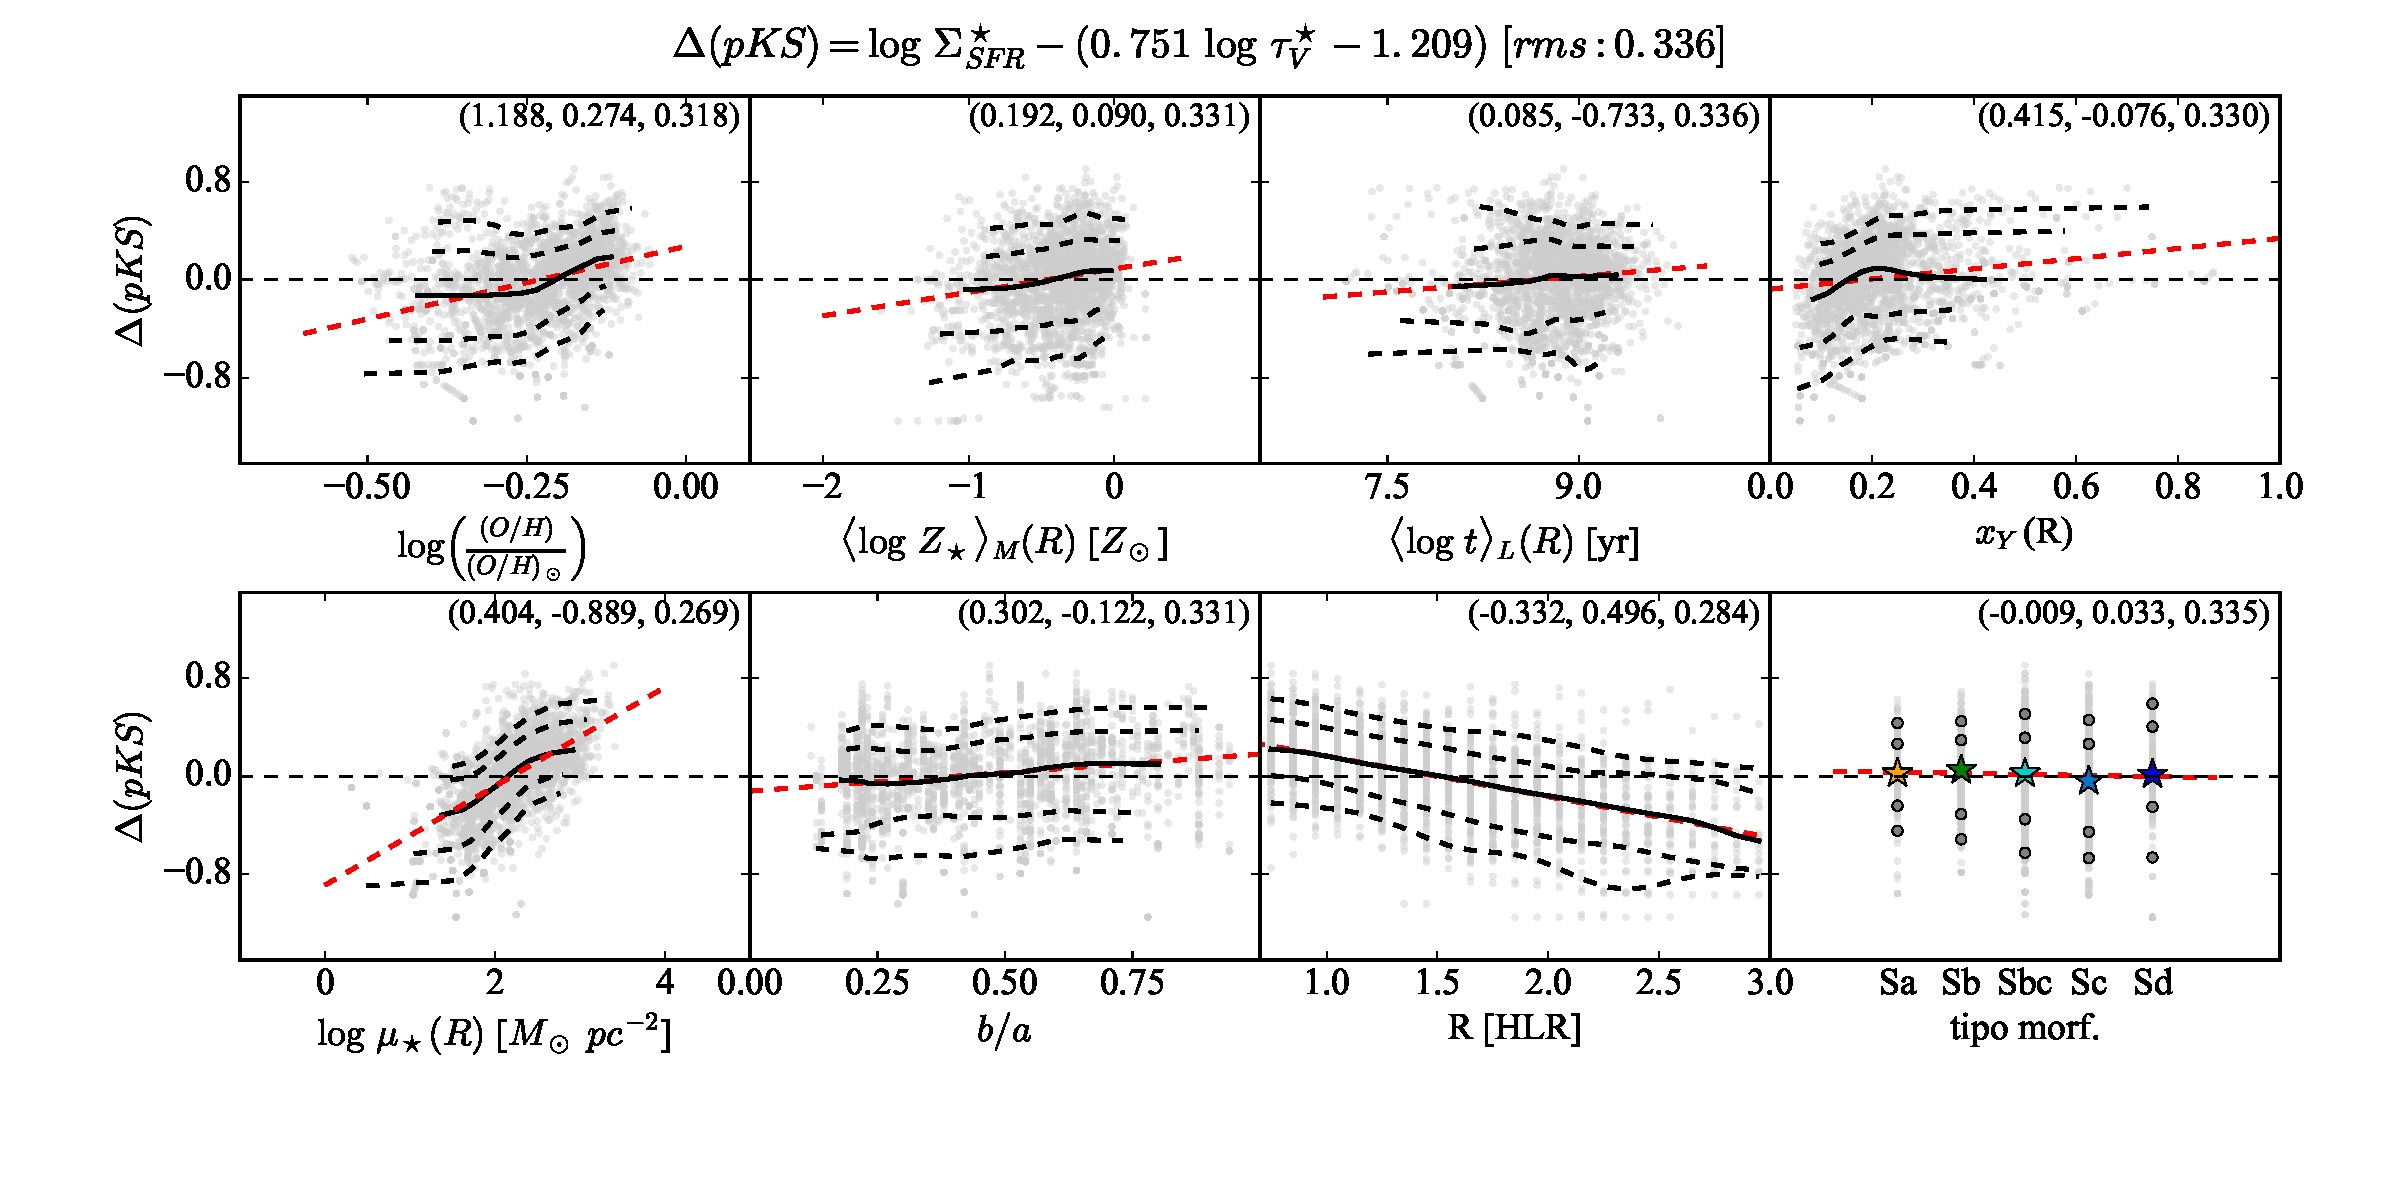
\includegraphics[width=0.99\textwidth]{figuras/deltapKS.pdf}
	\caption[Resíduos da {\em pseudo-KS}]
	{No eixo y de todos os painéis temos $\Delta(pKS)$ definido em \eqref{eq:DeltapKS}. \emph{Painéis
de a até d}: No eixo $x$ temos metalicidade nebular ($\log\ (O/H)$), metalicidade estelar média
pesada pela massa ($\meanM{\log Z_\star}$), idade média das populações estelares ($\meanL{\log
t_\star}$), fração em luz das populações estelares jovens ($x_Y$). \emph{Painéis de e até h}:
densidade superficial de massa estelar ($\log \mu_\star$), relação axial ($b/a$), raio e tipo
morfológico. Em cada painel as linhas pretas marcam a mediana (linha contínua) e os 5, 16, 64 e 95
percentis (linhas tracejadas). A linha tracejada vermelha representa a regressão linear da mediana,
cuja inclinação, o valor de y no qual há a interceptação do eixo x e o valor rms da distribuição
estão no canto superior direito. O número no canfo inferior esquerdo é o coeficiente de correlação
de Spearman.}
	\label{fig:deltapKS}
\end{figure}

Como próximo passo vamos tentar remover o espalhamento utilizando a regressão linear representada no
primeiro painel da Fig. \ref{fig:deltapKS}, ou seja, removendo o espalhamento causado pela
metalicidade nebular. Segundo o painel $a$ na Fig. \ref{fig:deltapKS} podemos aproximar a densidade
superficial da taxa de formação estelar como:
\begin{equation}
	\log\ \SigmaSFR(\tauVS, Z_{\mathrm{neb}})\ =\ 0.751 \log\ \tauVS + 1.188 \log
\left(\frac{(O/H)}{(O/H)_\odot}\right) - 0.935
	\label{eq:Delta1}
\end{equation}
\noindent onde incorporamos a metalicidade nebular à Eq. \eqref{eq:pKS_1stadj}. Definimos então um
novo $\Delta(pKS)$, alterando \eqref{eq:DeltapKS} utilizando \eqref{eq:Delta1}:
\begin{equation}
	\Delta(pKS)\ =\ \log\ \SigmaSFR - \log\ \SigmaSFR(\tauVS, Z_{\mathrm{neb}}).
\end{equation}
\noindent Este resultado pode ser observado na Fig. \ref{fig:deltapKS_noOH}. Vemos que apesar
de diminuir em uma maneira geral o espalhamento, vemos que a densidade superficial de massa estelar
continua cumprindo um papel importante nesta relação. Dessa forma, repetimos este último passo, mas
agora removendo o espalhamento causado por $\mu_\star$ ao invés da metalicidade nebular:
\begin{equation}
	\log\ \SigmaSFR(\tauVS, \mu_\star)\ =\ 0.751 \log\ \tauVS + 0.404 \log\ \mu_\star - 2.098
	\label{eq:Delta2}
\end{equation}
\noindent O novo valor de $\Delta(pKS)$ fica:
\begin{equation}
	\Delta(pKS)\ =\ \log \SigmaSFR - \log\ \SigmaSFR(\tauVS, \mu_\star).
\end{equation}
\noindent Como podemos ver na Fig. \ref{fig:deltapKS_noMcorSD}, após este processo o
espalhamento diminui consideravelmente na relação geral e em todas as outras variáveis, inclusive
com a metalicidade nebular. Esta propriedade, assim como $\mu_\star$, possui um gradiente no mesmo
sentido em relação ao raio, e talvez esse seja o motivo pelo qual quando removemos o espalhamento
causado por esta última resulte na diminuição do espalhamento causado pela primeira. Os efeitos com
idade, fração em de populações jovens, $b/a$ e morfologia serão estudados em um próximo passo de
nosso trabalho, principalmente no contexto do Cap. \ref{sec:difextin}. Parece que, em primeira
ordem, encontramos o mais forte causador do espalhamento da Fig. \ref{fig:pseudoKS}, painel
esquerdo. Na Fig. \ref{fig:pseudoKS_noscat} vemos o resultado desse processo na $pKS$.

\begin{figure}
	\centering
	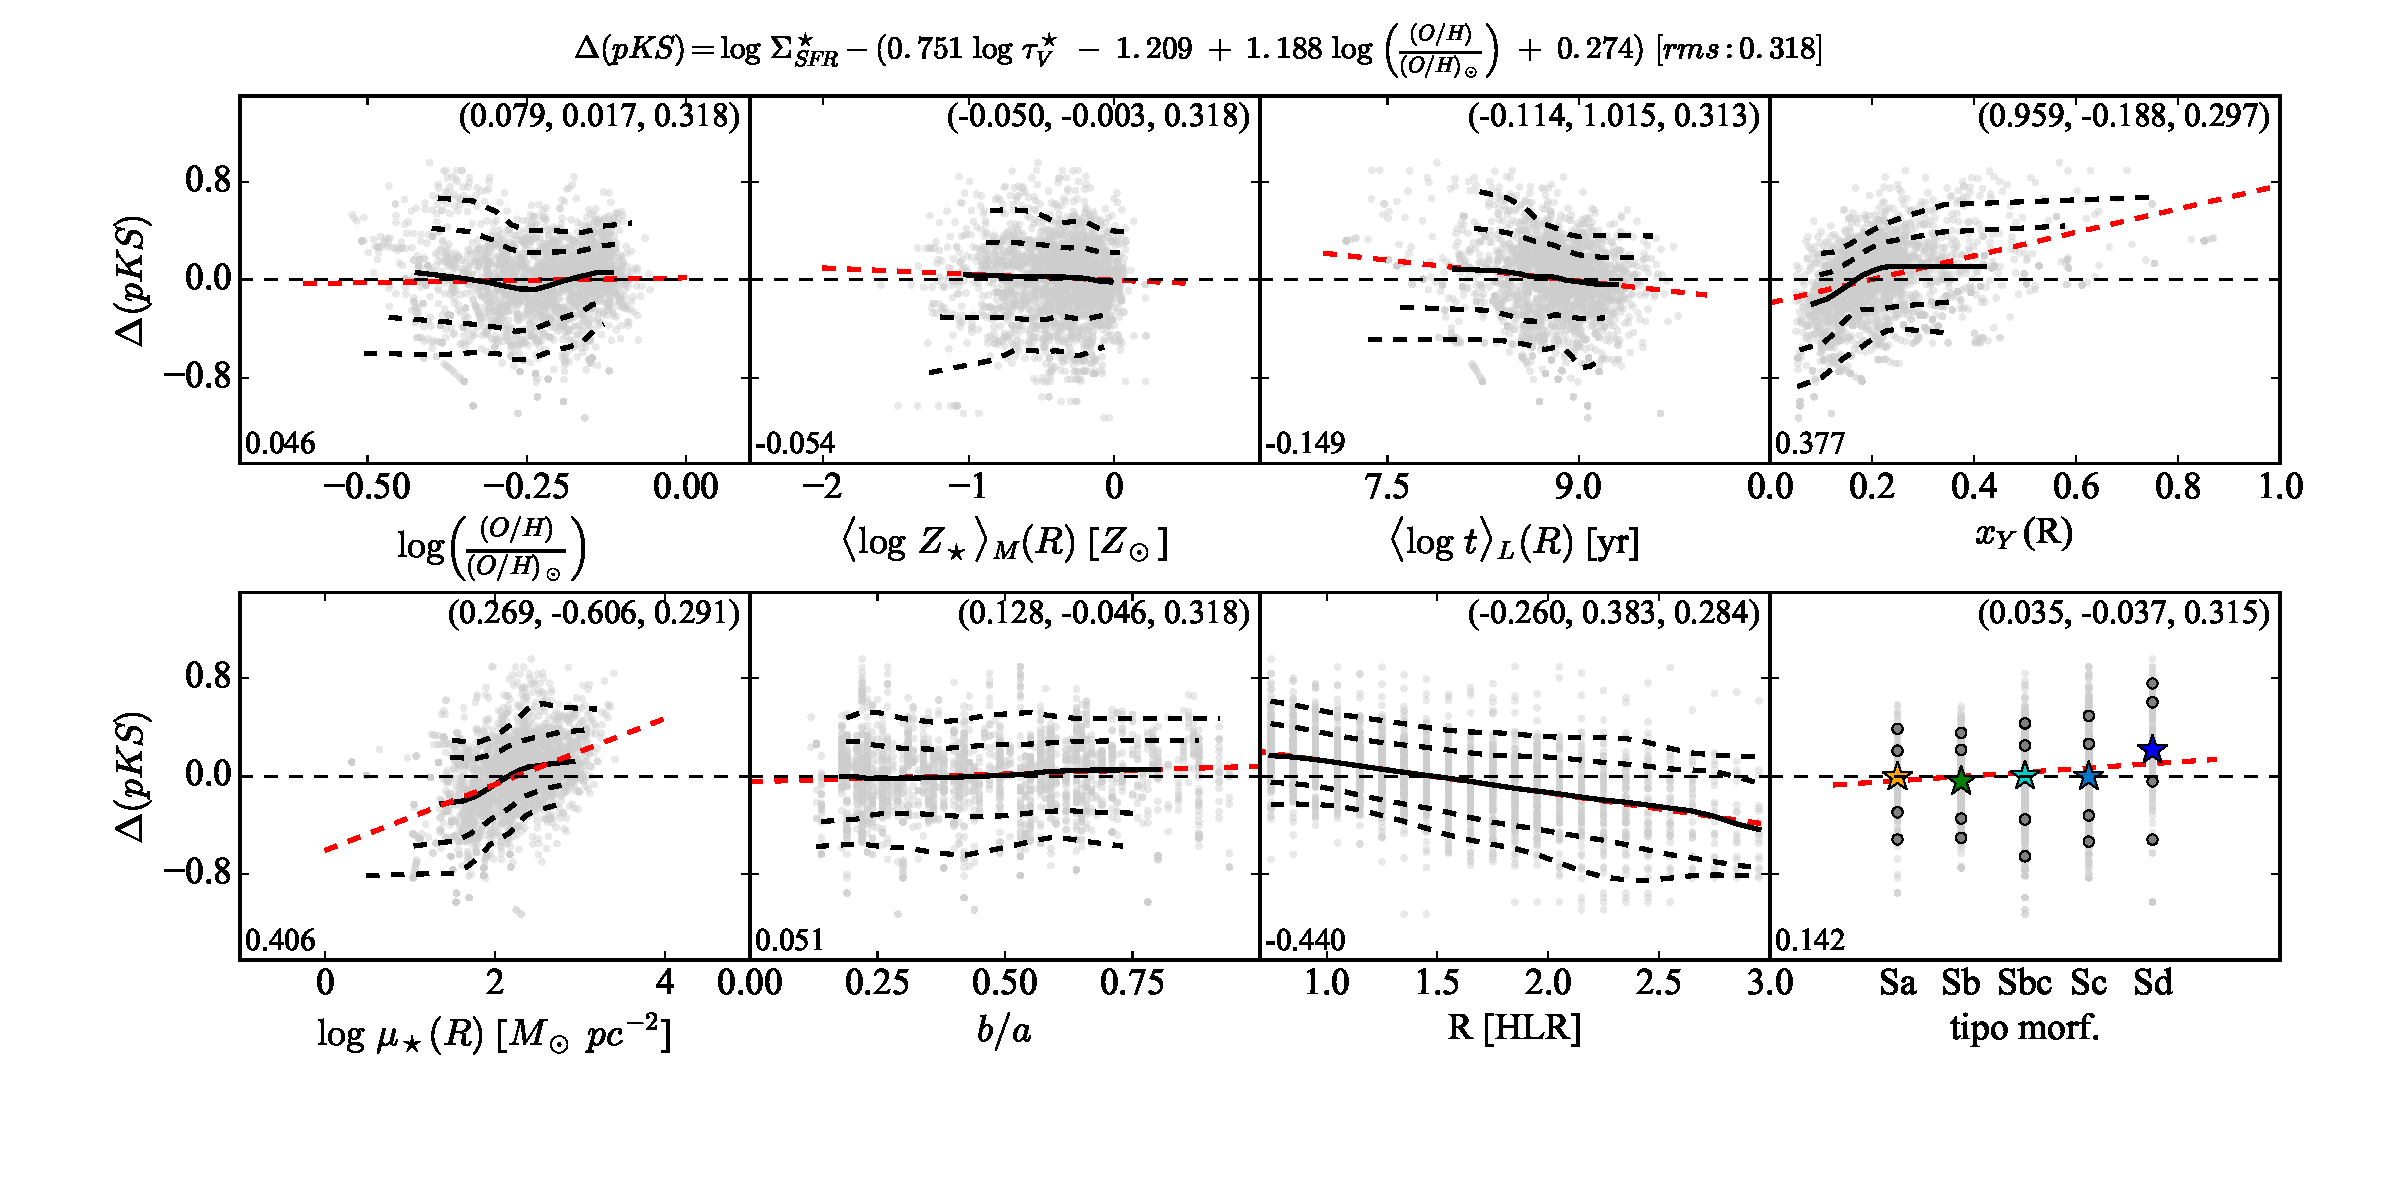
\includegraphics[width=0.99\textwidth]{figuras/deltapKS_noOH.pdf}
	\caption[Resíduos da {\em pseudo-KS} removendo o espalhamento com \left(\frac{(O/H)}{(O/H)_\odot}\right)]
	{Igual a Fig. \ref{fig:deltapKS}, mas removendo o espalhamento causado pela metalicidade
nebular, conforme a dependência mostrada no painel $a$.}
	\label{fig:deltapKS_noOH}
\end{figure}

\begin{figure}
	\centering
	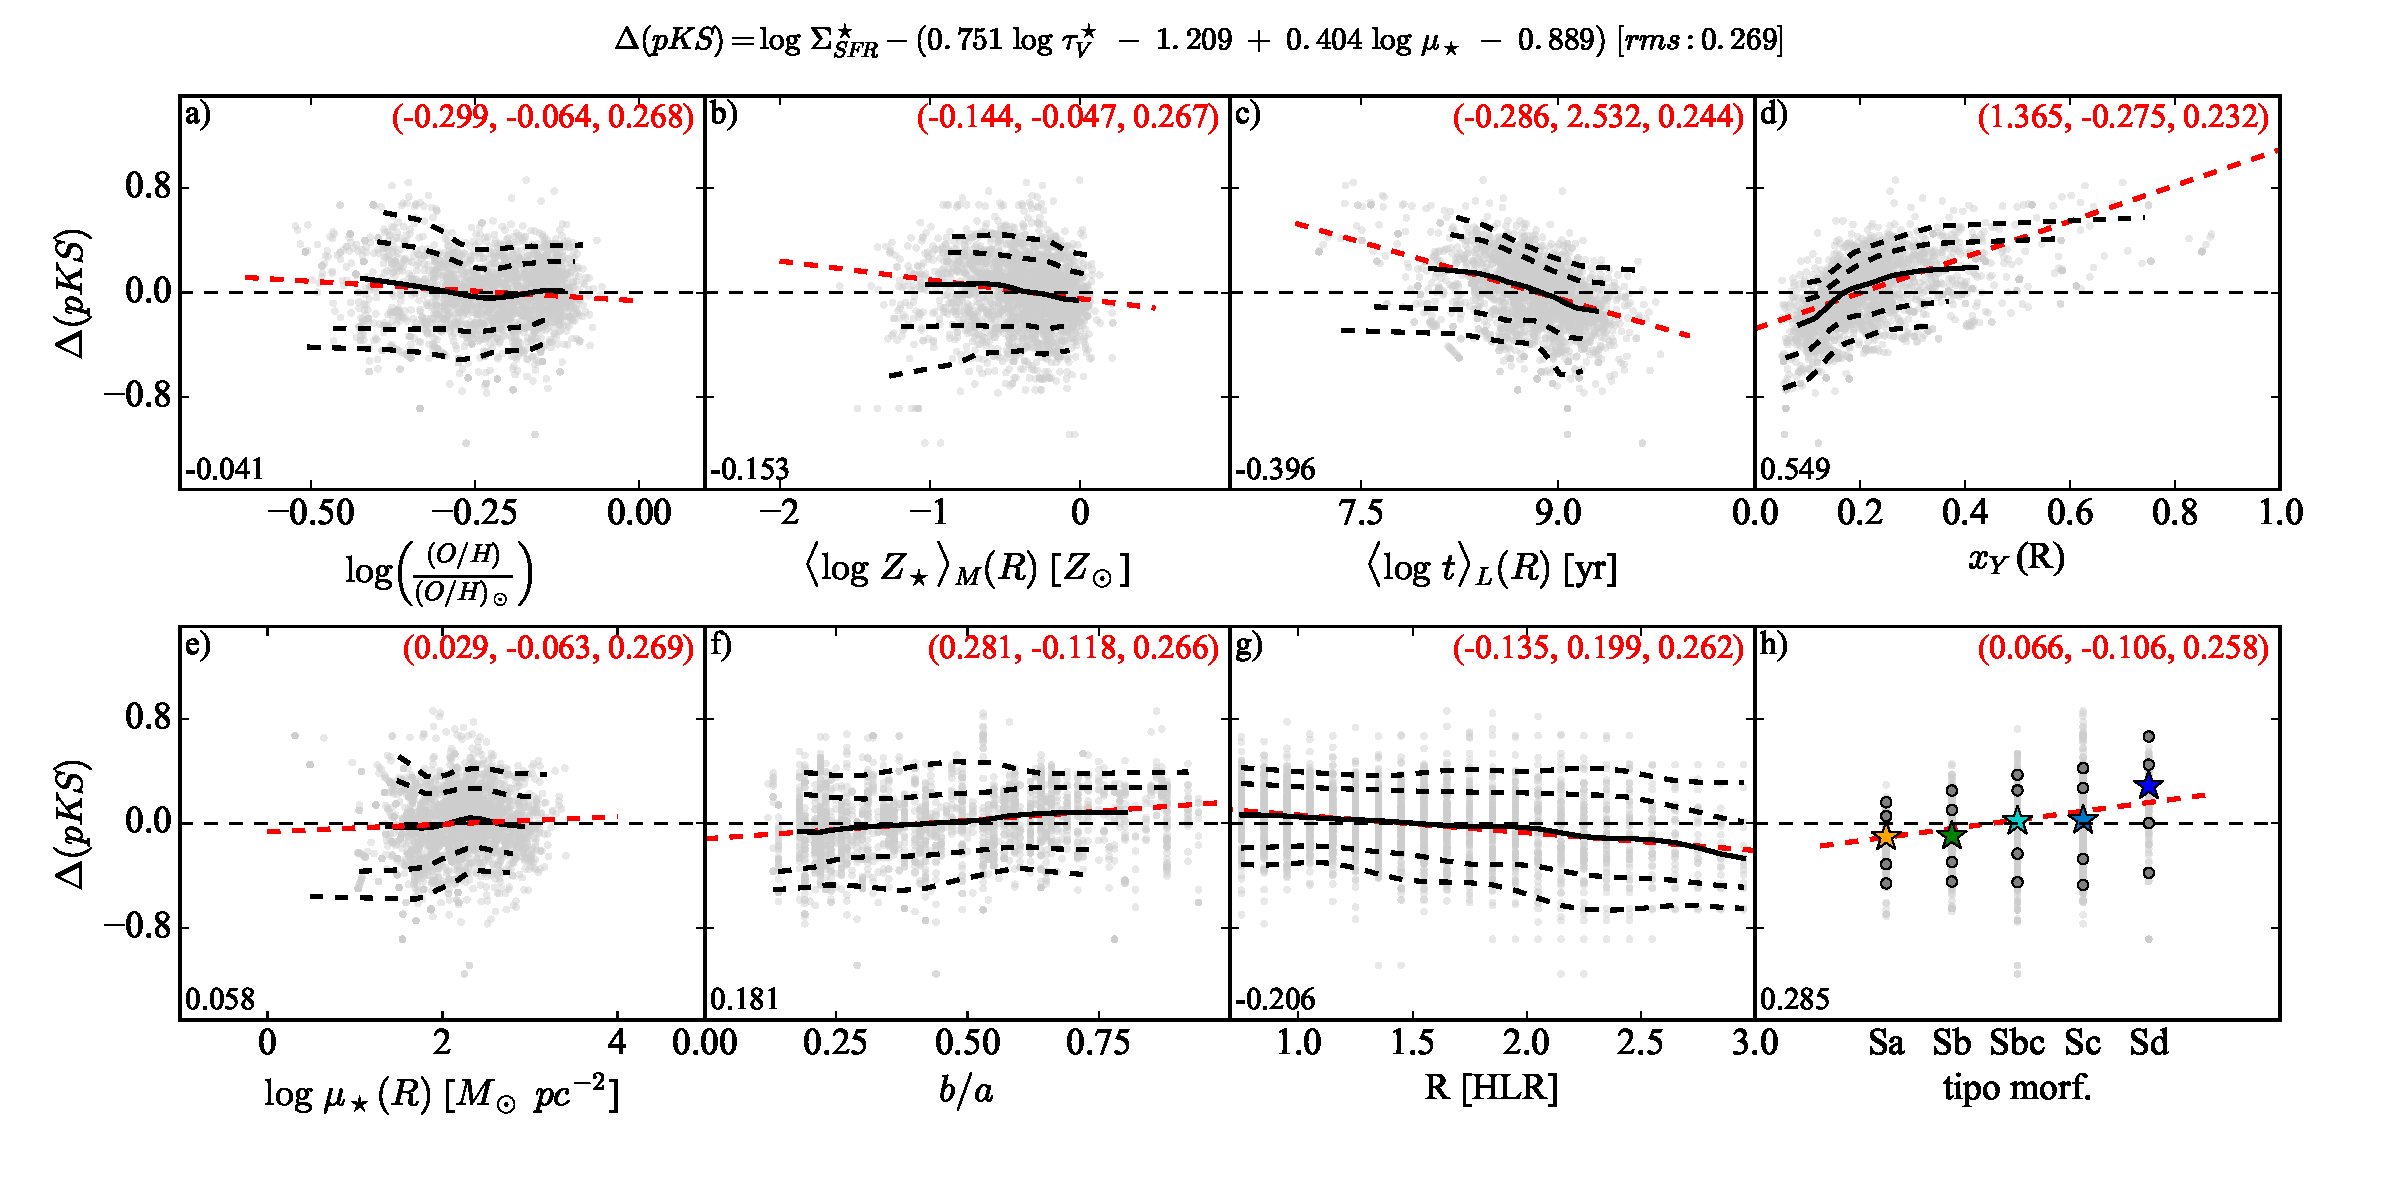
\includegraphics[width=0.99\textwidth]{figuras/deltapKS_noMcorSD.pdf}
	\caption[Resíduos da {\em pseudo-KS} removendo o espalhamento com $\mu_\star$]
	{Igual a Fig. \ref{fig:deltapKS_noOH}, mas removendo o espalhamento causado pela
densidade superficial de massa estelar, conforme a dependência mostrada no painel $e$ da Fig.
\ref{fig:deltapKS}.}
	\label{fig:deltapKS_noMcorSD}
\end{figure}

\begin{figure}
	\centering
	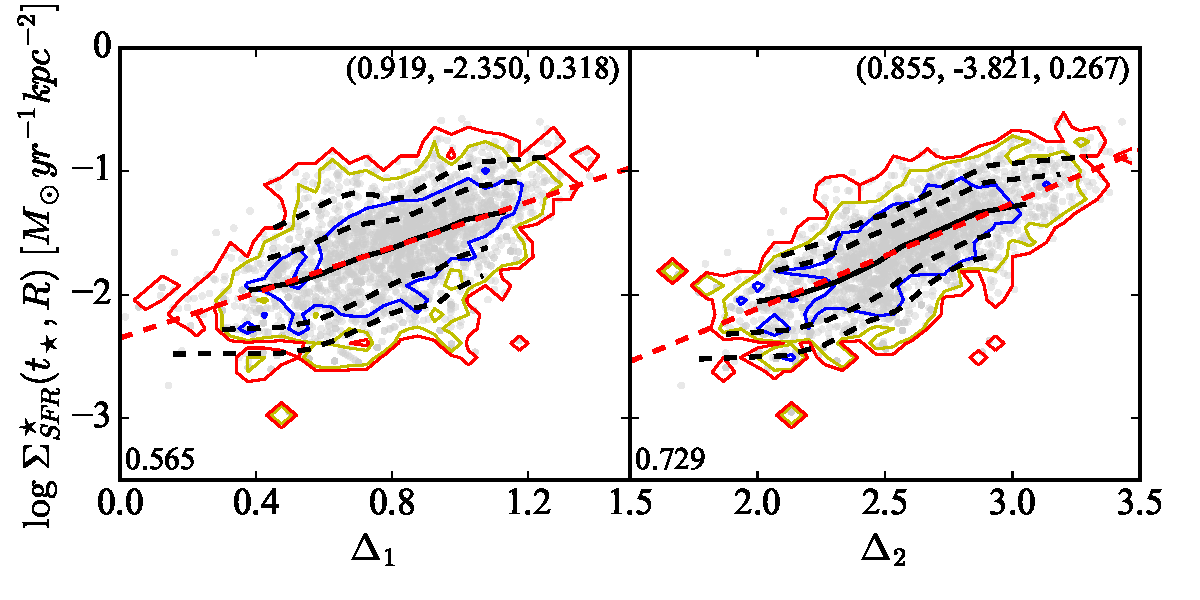
\includegraphics[width=0.8\textwidth]{figuras/pseudoKS_noscat.pdf}
	\caption[A {\em pseudo-KS} sem os principais causadores de espalhamento]
	{Igual a Fig. \ref{fig:pseudoKS}, mas agora usando no eixo $x$ os valores de $\log\ \SigmaSFR$
aproximados utilizando as Eqs. \ref{eq:Delta1} e \ref{eq:Delta2}, que se referem à remoção do
espalhamento causado pela metalicidade nebular e pela densidade superficial de massa estelar respectivamente.}
	\label{fig:pseudoKS_noscat}
\end{figure}

%Quando mudamos para os resíduos em torno da relação da direita na Fig. \ref{fig:pseudoKS} (Fig.
%\ref{fig:pseudoKSresid_neb}), o resultado é basicamente o mesmo, mas com uma dependência maior para
%a fração de luz das populações jovens e com uma dependência muito mais forte com a idade média das
%populações estelares. A participação da relação de semi-eixos ($b/a$) desaparece quase que
%completamente, mas aparece um pequeno desvio em relação às galáxias tipo Sd, mais jovens, menos
%evoluídas e com uma densidade superficial de formação estelar mais alta, na média, ao longo do
%disco.
%\begin{figure}
%	\centering
%	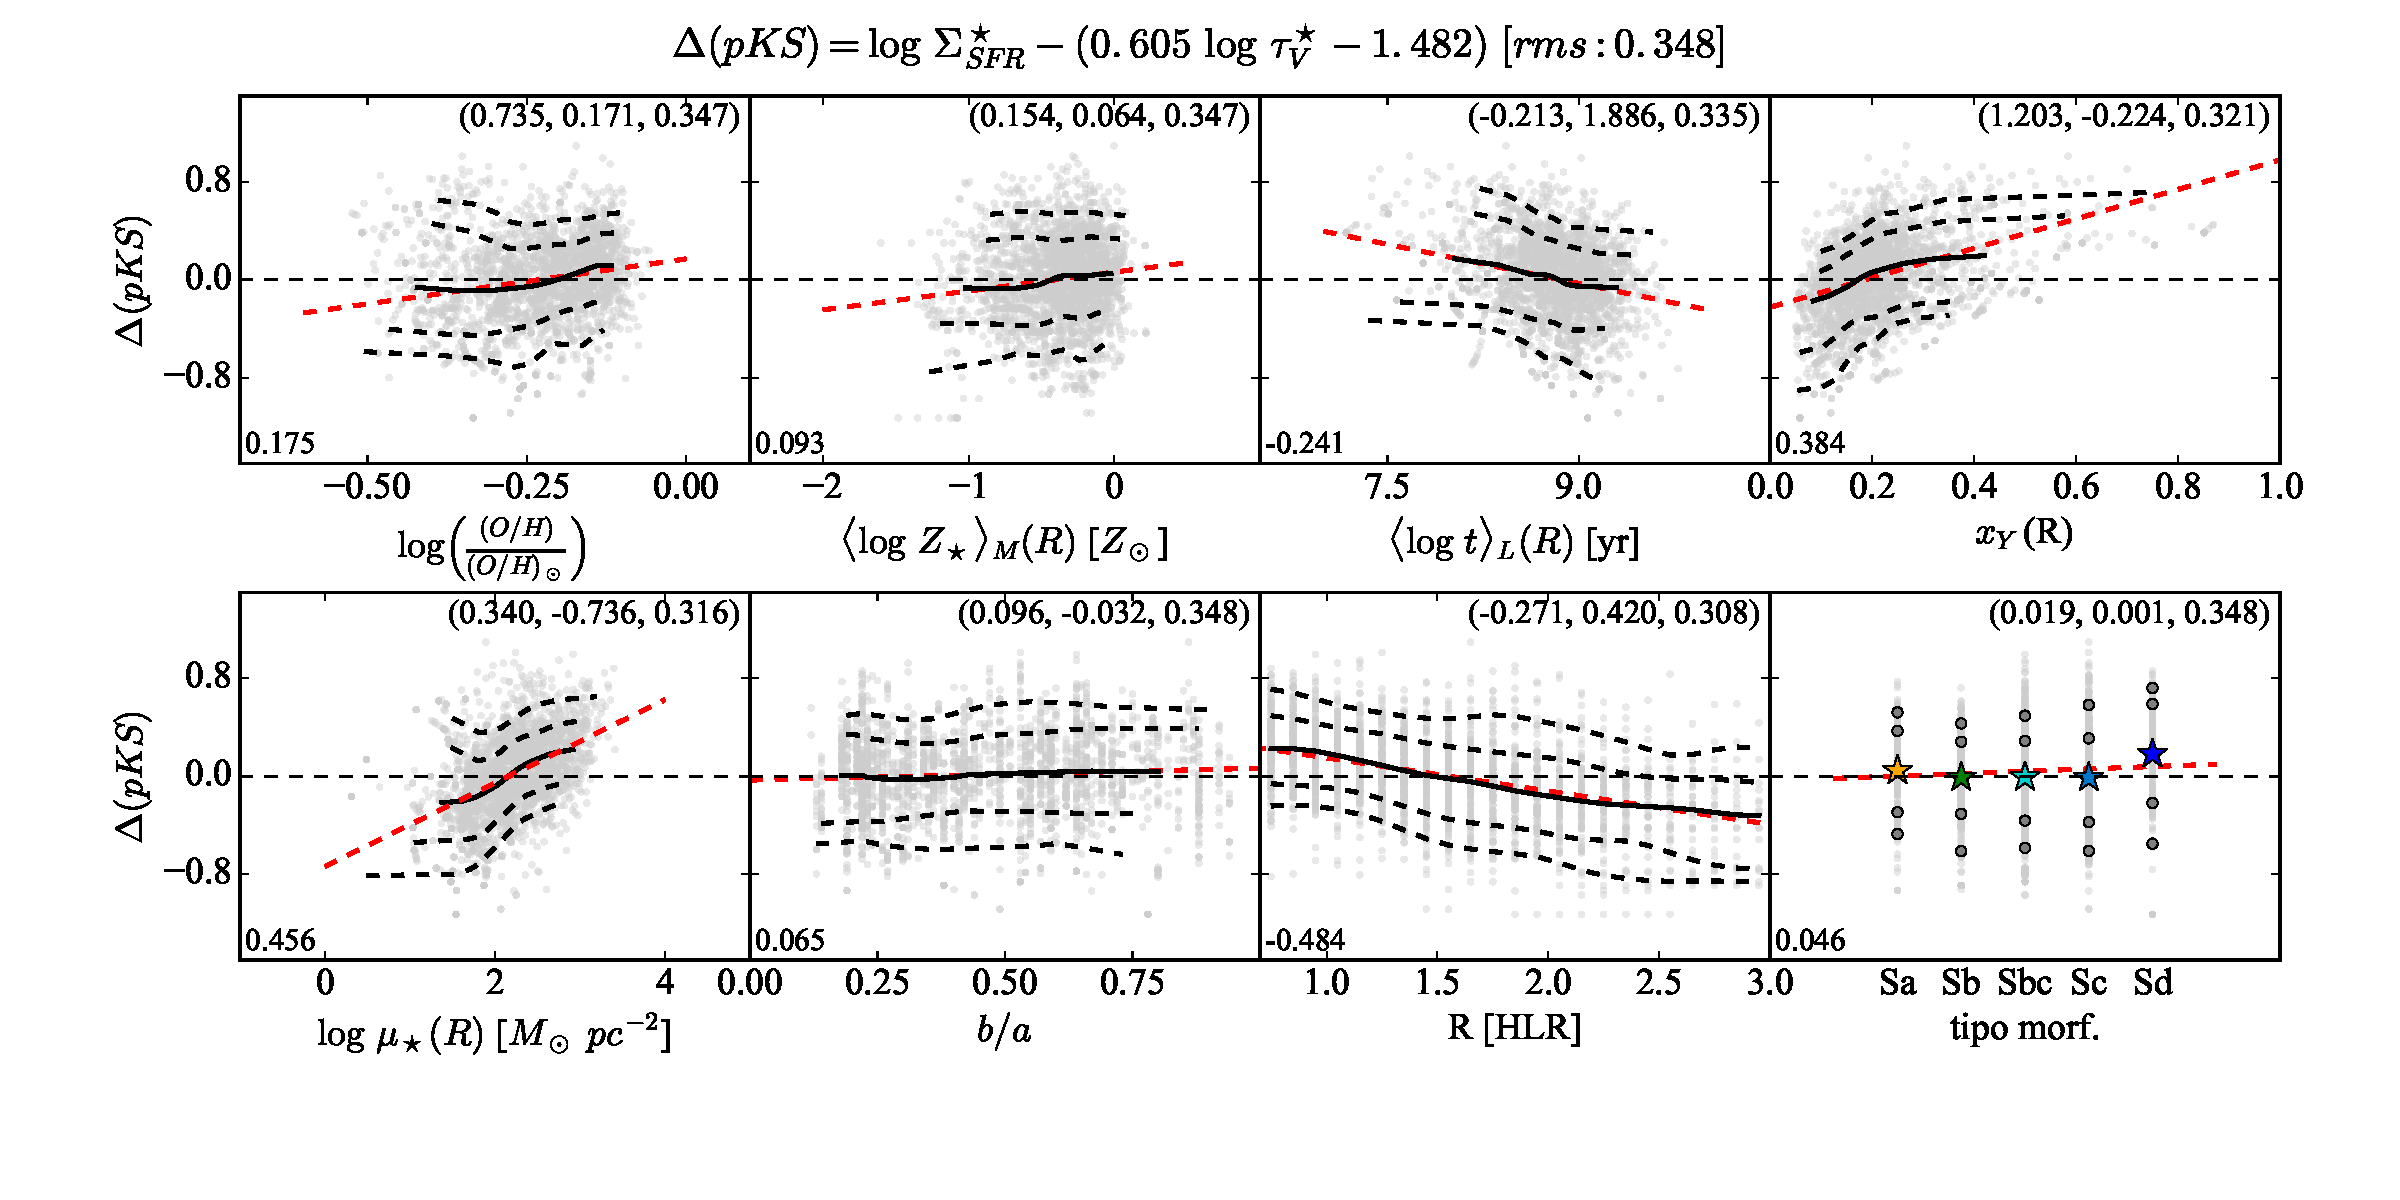
\includegraphics[width=0.99\textwidth]{figuras/deltapKS_neb.pdf}
%	\caption[Resíduos da {\em pseudo-KS}]
%	{Igual a Fig. \rf{fig:pseudoKSresid}, mas para a relação da direita na Fig. \ref{fig:pseudoKS}, ou
%seja, utilizando $\tauVN$ como o sinalizador de gás. }
%	\label{fig:pseudoKSresid_neb}
%\end{figure}

Diversos autores atualmente calculam e discutem a relação KS e a sua validade para diferentes
resoluções espaciais \citep[e.g., ][]{Kennicutt.etal.2007a, Leroy.etal.2012a,
Calzetti.Liu.Koda.2012a, Lada.etal.2013a, Tacconi.etal.2013a, Casasola.etal.2015a}. A inclinação
da KS (N = 1.4 em \eqref{eq:SFRKennicutt}) varia geralmente entre 1 e 2, dependendo da resolução
espacial observada (regiões \Hii, perfis radiais, galáxias integradas) ou do tipo de gás usado
(atômico, molecular ou a soma dos dois).

\section{Conversão de poeira em gás}
\label{sec:gasfrac:gas2dust}

Para converter poeira em gás primeiro precisamos da densidade superficial de poeira, que pode ser
conseguida partindo da definição de profundidade óptica:
\begin{eqnarray}
	\tau_{\mathrm{d}} &=& \sigma_{\mathrm{d}} \int n_{\mathrm{d}} dz =
	\frac{\sigma_{\mathrm{d}}}{m_{\mathrm{d}}}\times\Sigma_{\mathrm{d}}
	\\
	\Sigma_{\mathrm{d}} &=& \frac{m_{\mathrm{d}}}{\sigma_{\mathrm{d}}}\ \tau_{\mathrm{d}},
	\label{eq:sigmadust}
\end{eqnarray}
\noindent onde $\sigma_{\mathrm{d}}$ é seção de choque na banda V, $n_{\mathrm{d}}$ é o número de
grãos de poeira ao longo de uma profundidade $dz$ e $m_{\mathrm{d}}$ é a massa de um grão de poeira.
Substituindo \eqref{eq:sigmadust} em \eqref{eq:dust2gas} e assumindo $\tauV$ como $\tau_{\mathrm{d}}$ obtemos:
\begin{equation}
	\SigmaGas\ =\ \kappa \times \frac{m_{\mathrm{d}}}{\sigma_{\mathrm{d}}}\ \tauV. 
	\label{eq:dust2gas_tauV}
\end{equation}

A conversão de poeira em gás é dependente da metalicidade segundo podemos verificar em todas as
referências sobre o assunto. Vamos explorar a conversão de poeira em gás em BR13, onde os autores
identificam algumas variáveis que vamos utilizar:
\begin{eqnarray}
	\xi &=& \frac{\Sigma_{\mathrm{d}}}{\Sigma_Z} \\
	Z &=& \frac{\Sigma_Z}{\SigmaGas}  \\
	\delta_{\mathrm{DGR}} &=& \frac{\Sigma_{\mathrm{d}}}{\Sigma_Z}\ \frac{\Sigma_Z}{\SigmaGas}\ =\
\frac{\Sigma_{\mathrm{d}}}{\SigmaGas} = \xi Z,
	\label{eq:deltaDGR}
\end{eqnarray}
\noindent onde $\xi$ é a razão poeira-metais ({\em dust-to-metals}), Z é a metalicidade do gás e o
termo $\delta_{\mathrm{DGR}}$ é igual a $1/\kappa$. Utilizando \eqref{eq:deltaDGR} em
\eqref{eq:dust2gas_tauV} e fazendo $m_{\mathrm{d}}/\sigma_{\mathrm{d}} \approx 0.2\ g\ cm^{-2}$, que
corresponde ao tipo de poeira Galáctica (BR13), temos:
\begin{equation}
	\SigmaGas\ \approx\ 0.2 \frac{\tauV}{\delta_{\mathrm{DGR}}}\ [M_\odot \mathrm{pc}^{-2}].
	\label{eq:SigmaGasBR}
\end{equation}
Neste artigo os autores utilizaram dados de $\sim 70000$ galáxias {\em star-forming} do
\textit{SDSS}-DR7 e parametrizam $\delta_{\mathrm{DGR}}$ como a Eq. 28 de BR13:
\begin{equation}
	\delta_{\mathrm{DGR}}\ =\ (5.3 \times 10^{-3} - 1.1 \times 10^{-2})
\left(\frac{(O/H)}{(O/H)_\odot}\right),
	\label{eq:DGR_brinch_eq28}
\end{equation}
\noindent onde os fatores que multiplicam a metalicidade representam um intervalo onde esta
conversão é válida. O valor de $\delta_{\mathrm{DGR}}$ foi parametrizado utilizando as metalicidades
MPA/JHU\footnote{\href{http://wwwmpa.mpa-garching.mpg.de/SDSS/}{http://wwwmpa.mpa-garching.mpg.de/SDSS/}}
calculadas para o \SDSS. Para que possamos utilizar essa conversão, calibramos a abundância de
oxigênio de M13 com aquela utilizada no trabalho de BR13. Podemos ver na Fig. \ref{fig:calibZ} a
calibração feita utilizando 4 ajustes. Escolhemos utilizar o ajuste linear, que funciona tão bem
quanto ajustes de mais alta ordem. O ajuste da Fig. \ref{fig:calibZ} resulta em:
\begin{eqnarray}
	\label{eq:myZ}
	\log \left(\frac{(O/H)}{(O/H)_\odot}\right)_{MPA/JHU}\ &=&\ 2.016\ \log
\left(\frac{(O/H)}{(O/H)_\odot}\right)_{\mathrm{M}13} + 0.425 \\
	\label{eq:myDGR}	
	\delta_{\mathrm{DGR}}(\mathrm{M}13)\ &=&\ (1.4 - 2.9) \times 10^{-2}
\left(\frac{(O/H)}{(O/H)_\odot}\right)^{2.016}_{\mathrm{M}13},
\end{eqnarray}
\noindent onde multiplicamos os valores do intervalo em \eqref{eq:DGR_brinch_eq28} por $10^{0.425}$.

Na Fig. \label{fig:DGR_R} podemos ver o perfil radial médio de $\delta_{\mathrm{DGR}}$ para a
amostra definida neste trabalho. No fundo, esse é um perfil médio de $\log (O/H)$ na escala de M13
(Eq. \ref{eq:myZ}). Finalmente, substituindo \eqref{eq:myDGR} em \eqref{eq:SigmaGasBR} e utilizando
este resultado em \eqref{eq:fgas} podemos estimar frações de gás para galáxias do \CAL. A equação
final para fração de gás deste trabalho fica:
\begin{equation}
	f_{\mathrm{gas}}\ =\ \left(1 + \left(\frac{\mu_\star\ \delta_{\mathrm{DGR}}(\mathrm{M13})}{0.2\ 
\tauVS}\right)\right)^{-1}
	\label{eq:fgasthiswork}
\end{equation}

\begin{figure}
	\centering
	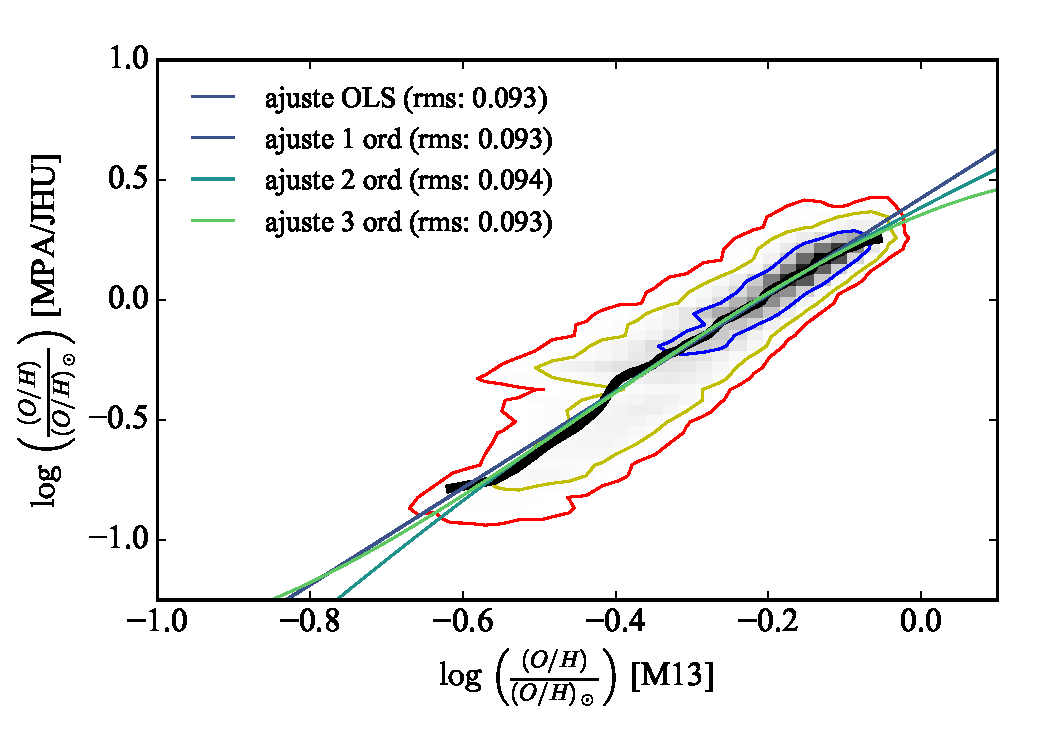
\includegraphics[width=0.9\textwidth]{figuras/logOH_ZnebMPA.pdf}
	\caption[Calibração das metalicidades]
	{Calibração da metalicidade nebular (abundância relativa de oxigênio) do grupo MPA/JHU com a de
M13. A linha preta contínua representa a mediana da distribuição, as outras linhas, pelas cores
indicadas na legenda, são regressões polinomiais de $1^\underline{a}$, $2^\underline{a}$ e
$3^\underline{a}$ ordem e o {\em OLS bisector} da distribuição. Os contornos marcam $1\sigma$,
$2\sigma$ e $3\sigma$ respectivamente.}
	\label{fig:calibZ}
\end{figure}

\begin{figure}
	\centering
	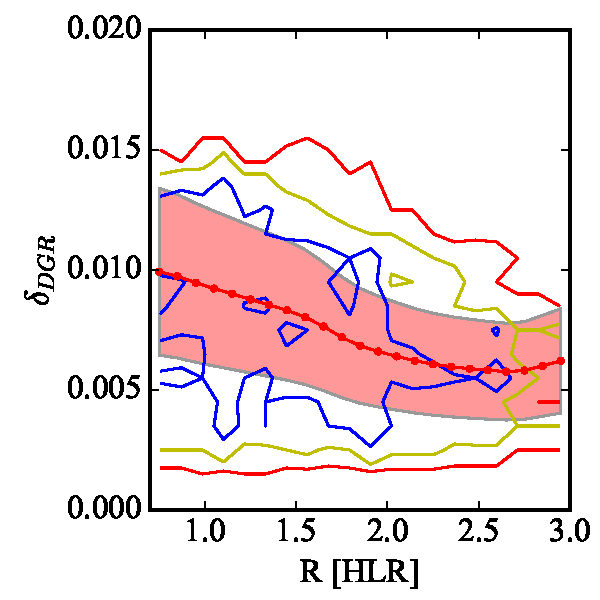
\includegraphics[width=0.5\textwidth]{figuras/DGR_R.pdf}
	\caption[Perfil radial de $\delta_{\mathrm{DGR}}]
	{Perfil radial médio de $\delta_{\mathrm{DGR}}$ definido em \eqref{eq:myDGR} para as 184 galáxias
da amostra. A área rachurada representa $\delta_{\mathrm{DGR}}$ calculado para os valores máximo e
mínimo do intervalo definido por BR13. Os contornos marcam $1\sigma$, $2\sigma$ e $3\sigma$
respectivamente.}
	\label{fig:DGR_R}
\end{figure}

\subsection{Analisando a conversão}
\label{sec:gasfrac:gas2dust:analisradperf}

Como não possuímos medidas diretas de gás para comparar com os valores estimados aqui, vamos
utilizar uma forma indireta invertendo \eqref{eq:SFRKennicutt} para calcular $\SigmaGas$ a
partir da KS, desta forma obtemos:
\begin{eqnarray}
	\SigmaGas^{\mathrm{KS}} &=& 374.02\ \left(\frac{\SigmaSFR}{M_\odot\ \mathrm{yr}^{-1}\
\mathrm{kpc}^{-2}}\right)^{\frac{1}{1.4}}\ M_\odot\ \mathrm{pc}^{-2} \\
	\label{eq:SigmaGasKenn}
	f_{\mathrm{gas}}^{\mathrm{KS}} &=& \frac{1}{1 +
	\left(\frac{\mu_\star}{\SigmaGas^{\mathrm{KS}}}\right)}.
	\label{eq:fGasKenn}
\end{eqnarray}
\noindent Juntamente produzimos a mesma versão destas variáveis, mas substituindo os $\SigmaSFR$ e
$\tauVS$ para $\SigmaSFRN$ e $\tauVN$.

A Fig. \ref{fig:propsGasR} mostra os perfis radiais médios de $\SigmaGas$ e $f_{\mathrm{gas}}$.
Apesar da divergência entre os perfis de $\SigmaGas$ quanto ao comportamento ao longo do raio, a
fração de gás parece ser um resultado mais robusto, graças a influência de densidade superficial de
massa estelar ($\mu_\star$). Em todos os casos vemos que $f_{\mathrm{gas}}$ cresce de dentro para
fora, sendo uns poucos porcentos nas regiões internas dos discos e atingindo $\sim 20\%$ nas partes
externas (R > 2 HLR).

\begin{figure}
	\centering
	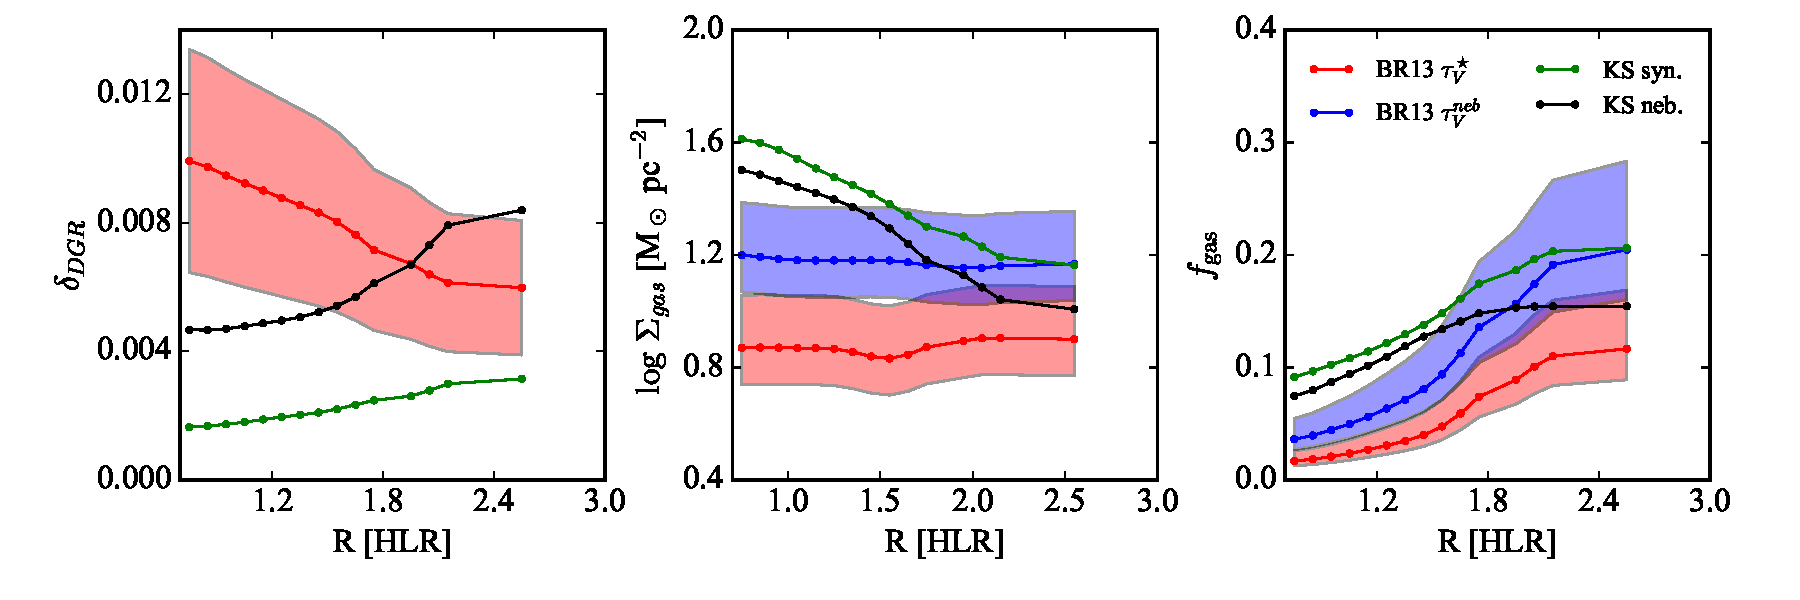
\includegraphics[width=0.9\textwidth]{figuras/gas_R.pdf}
	\caption[Perfis radiais de $\SigmaGas$ e $f_{\mathrm{gas}}$]
	{Perfis radiais médios da densidade superficial de massa de gás ($\SigmaGas$) e fração de gás
($f_{\mathrm{gas}}$). A área hachurada representa o intervalo definido em \eqref{eq:myDGR}. Em azul
e vermelho temos a conversão de poeira em gás utilizando a conversão \eqref{eq:SigmaGasBR} com
$\delta_{\mathrm{DGR}}$ definido em \eqref{eq:myDGR}, utilizando $\tauVN$ e $\tauVS$
respectivamente. Em verde e preto temos as variáveis definidas no início desta seção, invertendo a
lei de KS, utilizando $\SigmaSFR$ e $\SigmaSFRN$ respectivamente.}
	\label{fig:propsGasR}
\end{figure}

Na Fig. \ref{fig:histoGas} vemos os histogramas das variáveis calculadas nessa seção e nas Figs.
\ref{fig:propsSigmaGas} e \ref{fig:propsfGas} vemos $\SigmaGas$ e $f_{\mathrm{gas}}$ versus algumas
propriedades. O código de cores em todos os gráficos segue àquele definido na Fig.
\ref{fig:propsGasR}. Para $\SigmaGas$ vemos que os resultados são bastante diferentes quando
comparamos os valores calculados pelo método de conversão de poeira em absorção (utilizando um
$\delta_{\mathrm{DGR}}$) e aqueles através da inversão da lei de KS (Eqs. \ref{eq:SigmaGasKenn} e
\ref{eq:fGasKenn}). Já quando observamos frações de gás vemos que os resultados são mais
parecidos.

\begin{figure}
	\centering
	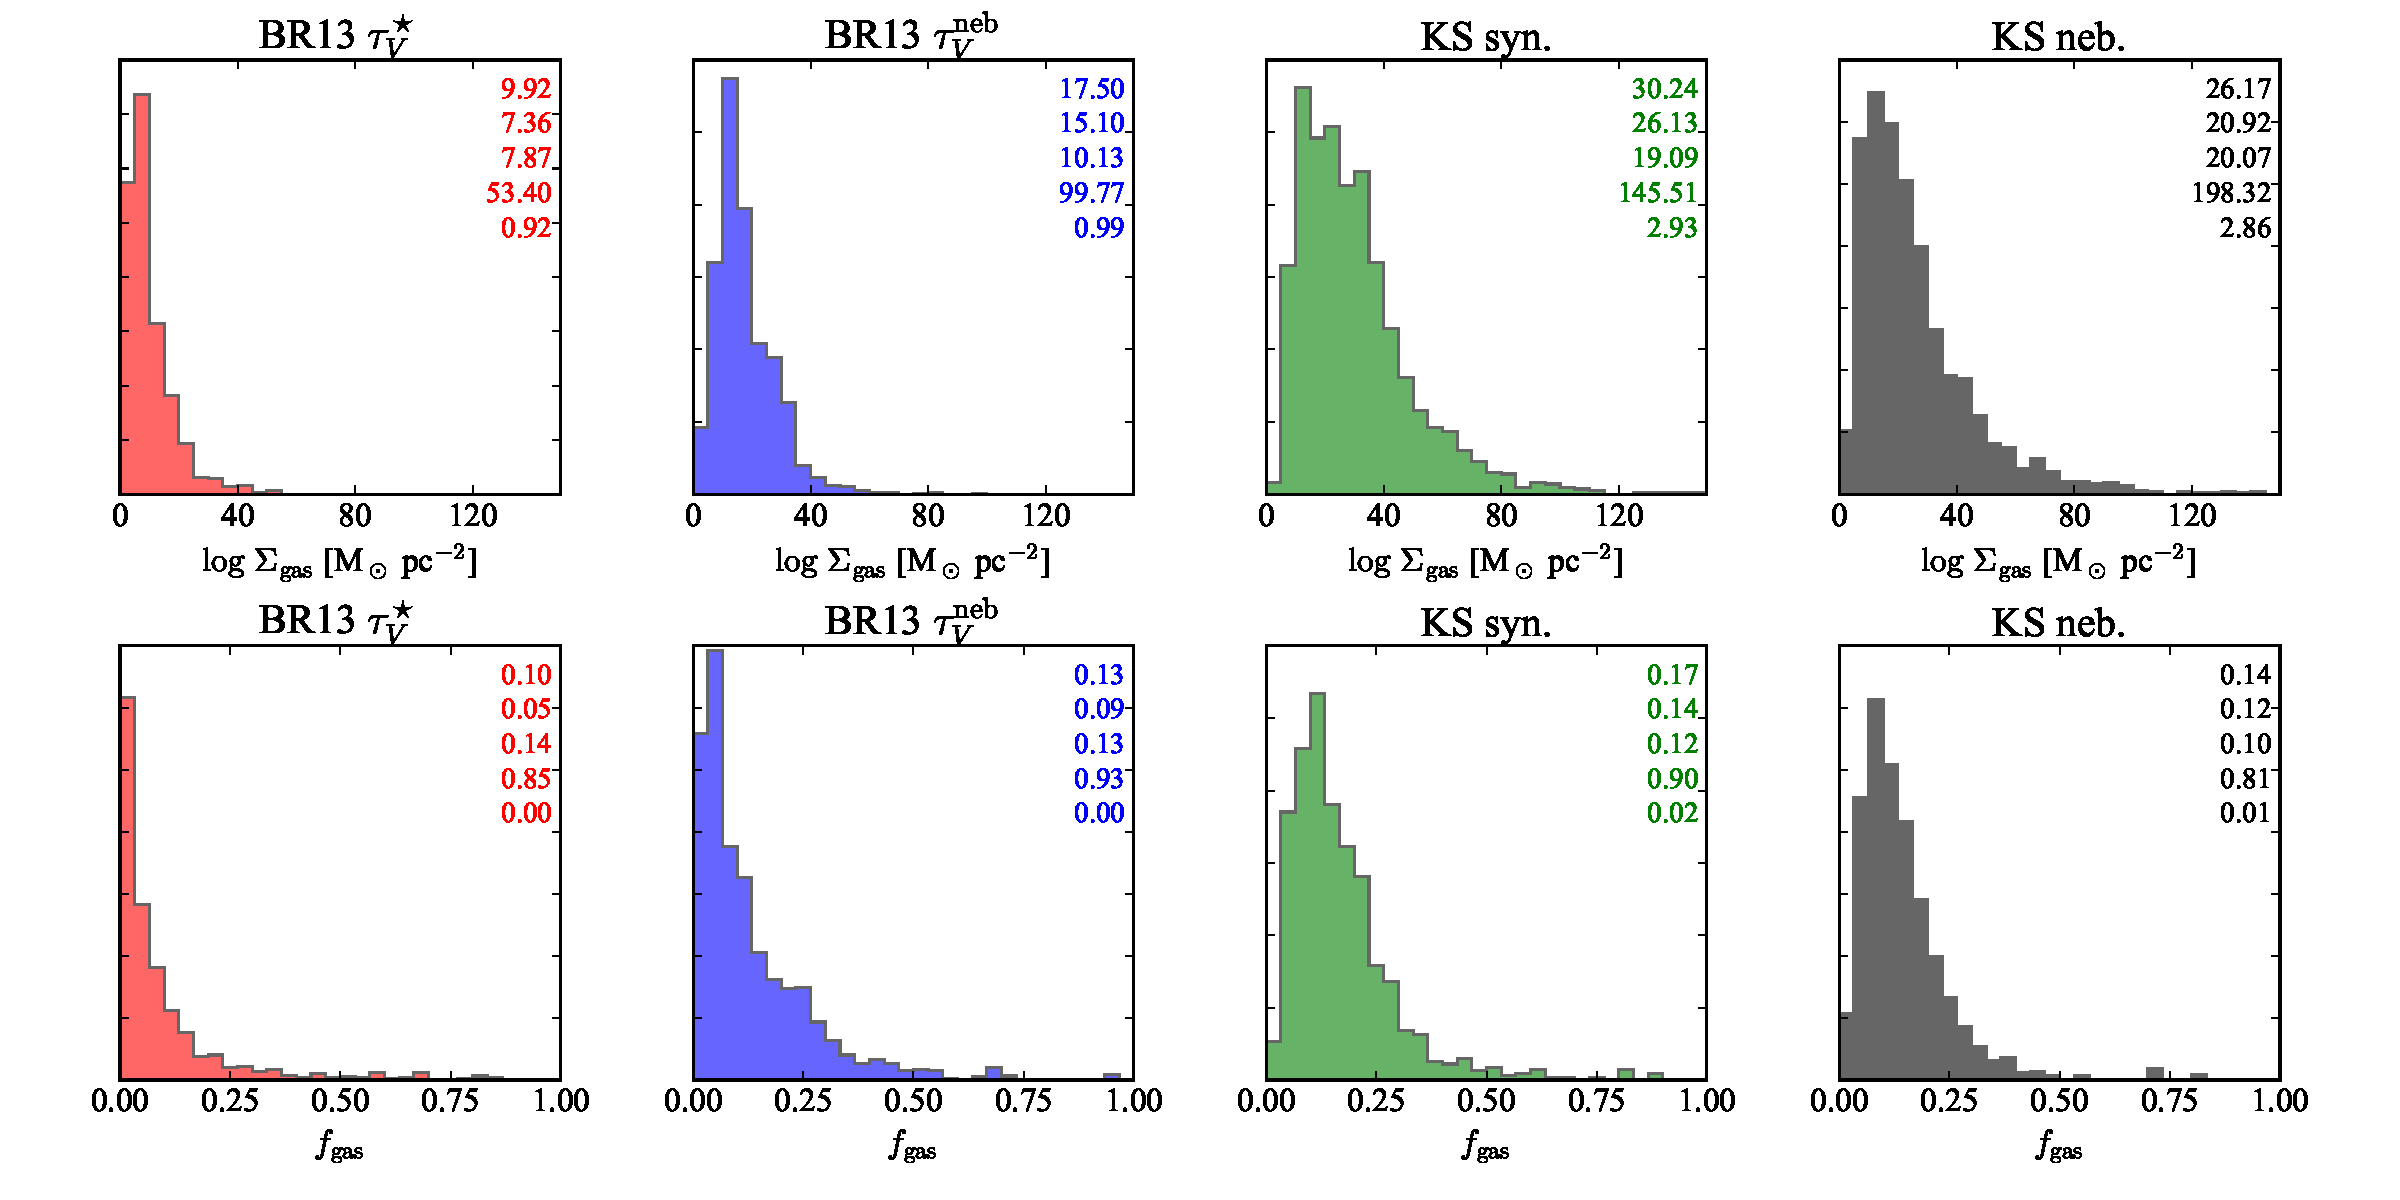
\includegraphics[width=0.99\textwidth]{figuras/histo_gas_R.pdf}
	\caption[Histogramas de $\SigmaGas$ e $f_{\mathrm{gas}}$]
	{Histogramas de $\SigmaGas$ e $f_{\mathrm{gas}}$ calculadas das diferentes formas especificadas
na Sec. \ref{sec:gasfrac:gas2dust:analisradperf}. As cores de cada histograma seguem àquelas
definidas na Fig. \ref{fig:propsGasR}. Os valores nos cantos são os mesmos encontrados em todos os
histogramas deste trabalho: média, mediana, desvio padrão, máximo e mínimo.}
	\label{fig:histoGas}
\end{figure}

\begin{figure}
	\centering
 	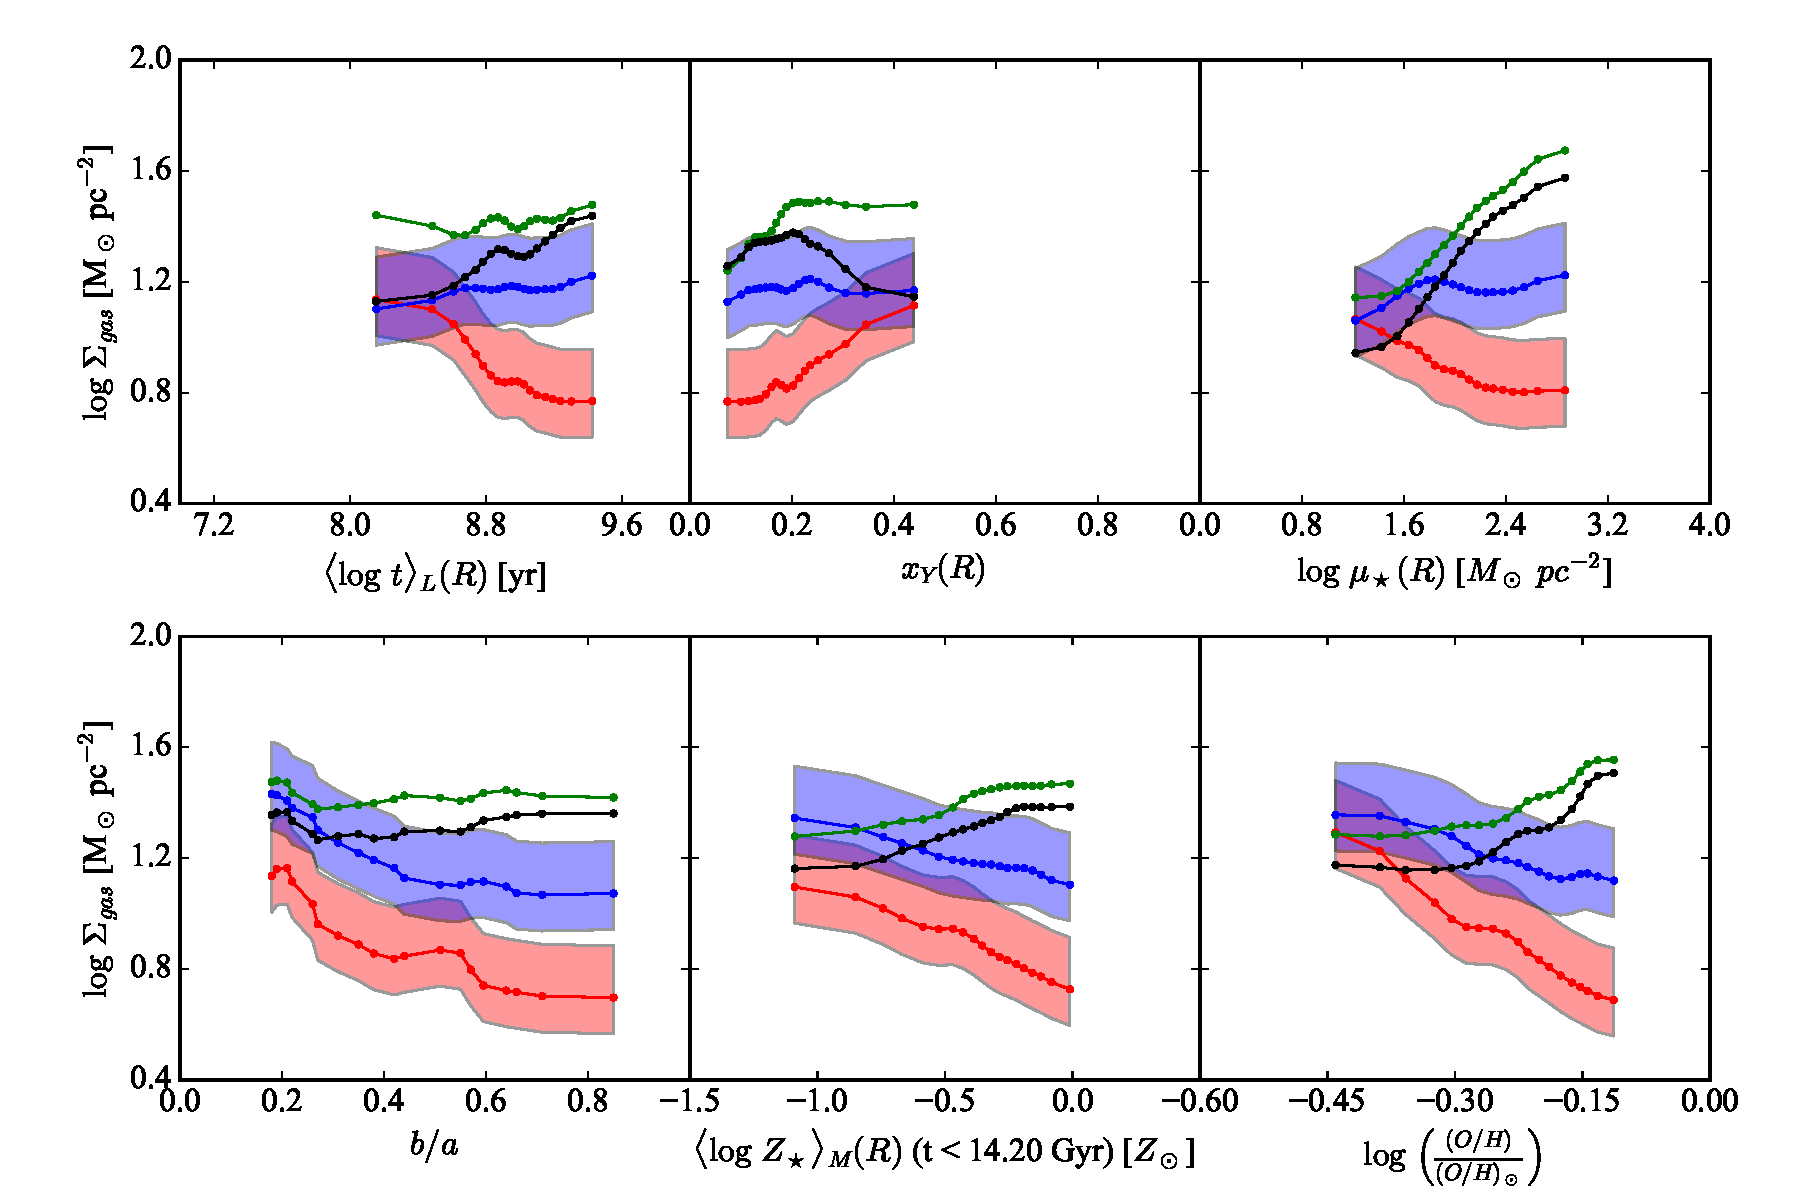
\includegraphics[width=0.99\textwidth]{figuras/props_SigmaGas.pdf}
 	\caption[Propriedades físicas e $\SigmaGas$]
 	{Densidade superficial de massa de gás ($\SigmaGas$) contra idade média das populações estelares,
fração em luz das populações jovens, densidade superficial de massa estelar, todos na primeira
fileira e, na segunda fileira, relação de semi-eixos, metalicidade média das populações estelares
pesada pela massa e metalicidade nebular.}
	\label{fig:propsSigmaGas}
\end{figure}

\begin{figure}
	\centering
 	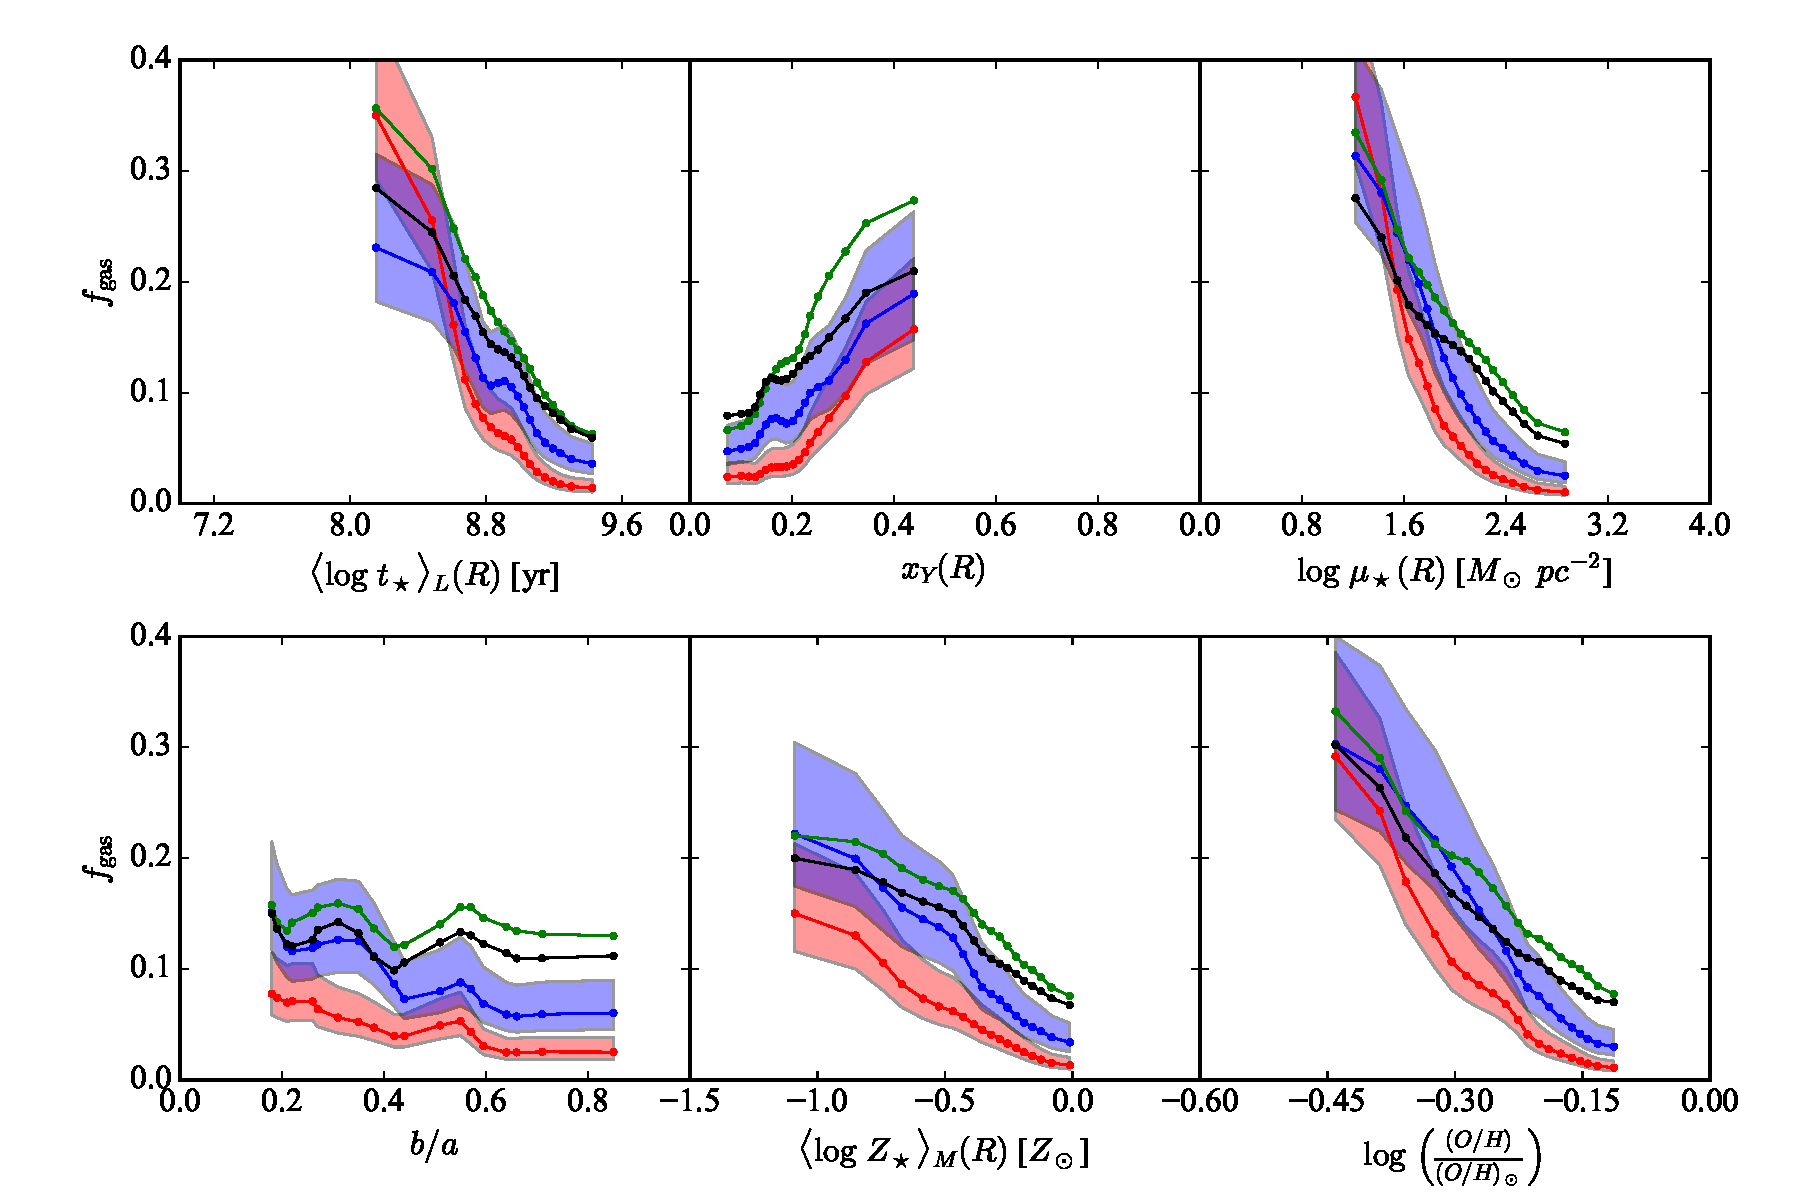
\includegraphics[width=0.99\textwidth]{figuras/props_fGas.pdf}
 	\caption[Propriedades físicas e $f_{\mathrm{gas}}$]
 	{Igual a Fig. \ref{fig:propsSigmaGas}, mas para a fração de gás.}
 	\label{fig:propsfGas}
\end{figure} 

Fechamos esta seção com a relação KS criada a partir dos valores de $\SigmaGas$ utilizando a
conversão de BR13 (Fig. \ref{fig:KS}). Basicamente o resultado é: essa conversão não está
``melhorando'' os resultados na direção de uma relação mais inclinada do que a relação original, que
seria o caso de ir em direção à relação de KS, que tem uma inclinação maior (1.4). Os resíduos de
metalicidade na relação $pKS$ (Fig. \ref{fig:deltapKS}, primeiro painel na primeira fila) estão indo
para a direção contrária a direção que deveria ter no caso de usar a conversão de poeira para gás
assumindo \eqref{eq:SigmaGasBR} para chegar em uma relação de KS \eqref{eq:SFRKennicutt}.

\begin{figure}
	\centering
	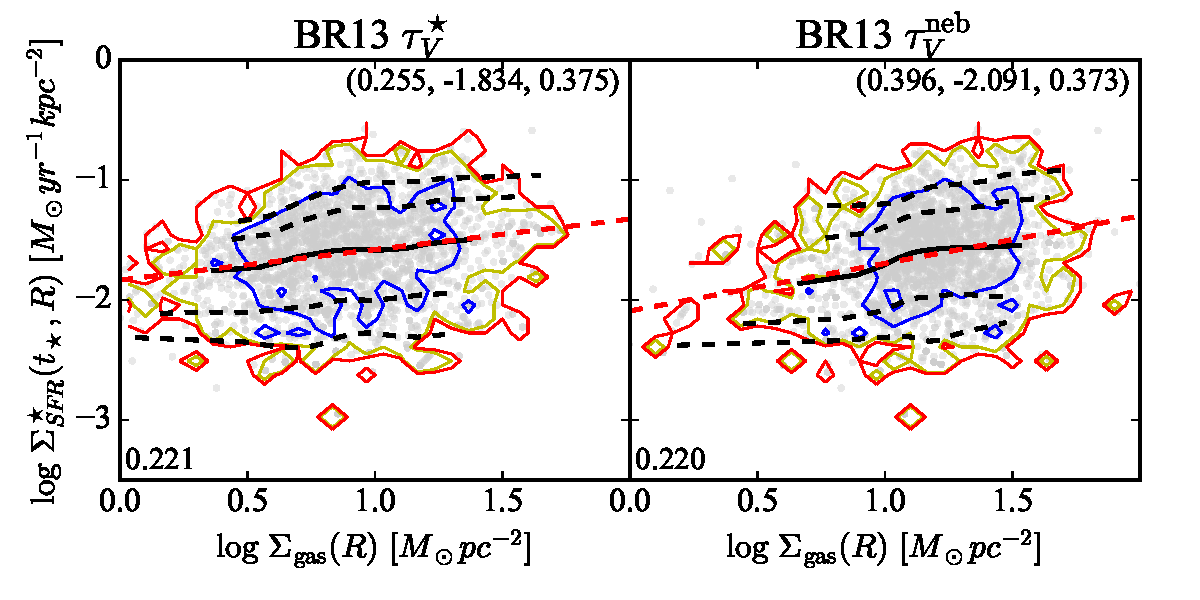
\includegraphics[width=0.99\textwidth]{figuras/KS.pdf}
	\caption[Relação de Kennicut-Schmidt]
	{Igual a Fig. \ref{fig:pseudoKS} mas substituindo o eixo $x$ para o valor da densidade superficial
de massa de gás calculado a partir da conversão de BR13 utilizando $\tauVS$ ({\em painel esquerdo})
e $\tauVN$ ({\em painel direito}).}
	\label{fig:KS}
\end{figure}

\section{Perspectivas e próximos passos}
\label{sec:gasfrac:nextsteps}

Nossa principal dificuldade nessa etapa é a falta de medidas diretas de gás para as mesmas regiões
avaliadas, de forma a parametrizar uma conversão. A conversão de BR13 parece foi definida como
somente dependente da metalicidade \eqref{eq:DGR_brinch_eq28} mas na Sec. \ref{sec:gasfrac:KS:resid}
verificamos que outras variáveis afetam a $pKS$, principalmente a densidade superficial de massa
estelar ($\mu_\star$). Precisamos estudar melhor esta relação também substituindo $\tauVS$ por $\tauVN$ e
também a explorar as diferenças entre $\tauVS$, $\tauVN$, $\tauISM$ e $\tauBC$ e suas influências na
relação $pKS$. 

O desvio padrão da relação KS construída utilizando $\SigmaGas$ vindo da conversão de
BR13 é próximo a 0.4 dex e, após a conversão, a inclinação da reta diminui, o que vai na direção
contrária ao que imaginaríamos assumindo uma relação KS com inclinação $\sim 1.4$. 

Um próximo passo também é adotar um outro tipo de abordagem, considerando a eficiência da
formação estelar (transformação de gás em estrelas), utilizando a relação:
\begin{equation}
	\mathrm{SFE} = \frac{\Sigma_{\mathrm{SFR}}}{\Sigma_{\mathrm{gas}}} = \frac{1}{t_{\mathrm{dep}}},
	\label{eq:SFE}
\end{equation}
\noindent onde SFE vem de {\em star-formation efficiency} e $t_{\mathrm{dep}}$, que é o inverso da
eficiência, é o tempo de depleção do gás, que nos dá uma ideia da escala de tempo em que a galáxia
consome todo o gás com a taxa em que está formando estrelas. Um exemplo desse tipo de análise pode
ser visto na Fig. \ref{fig:tdep}, onde utilizamos $\SigmaGas$ proveniente dos métodos utilizados
nesse capítulo para verificar o tempo de depleção do gás, o qual nos diz o tempo médio no qual o
gás é consumido.

\begin{figure}
	\centering
	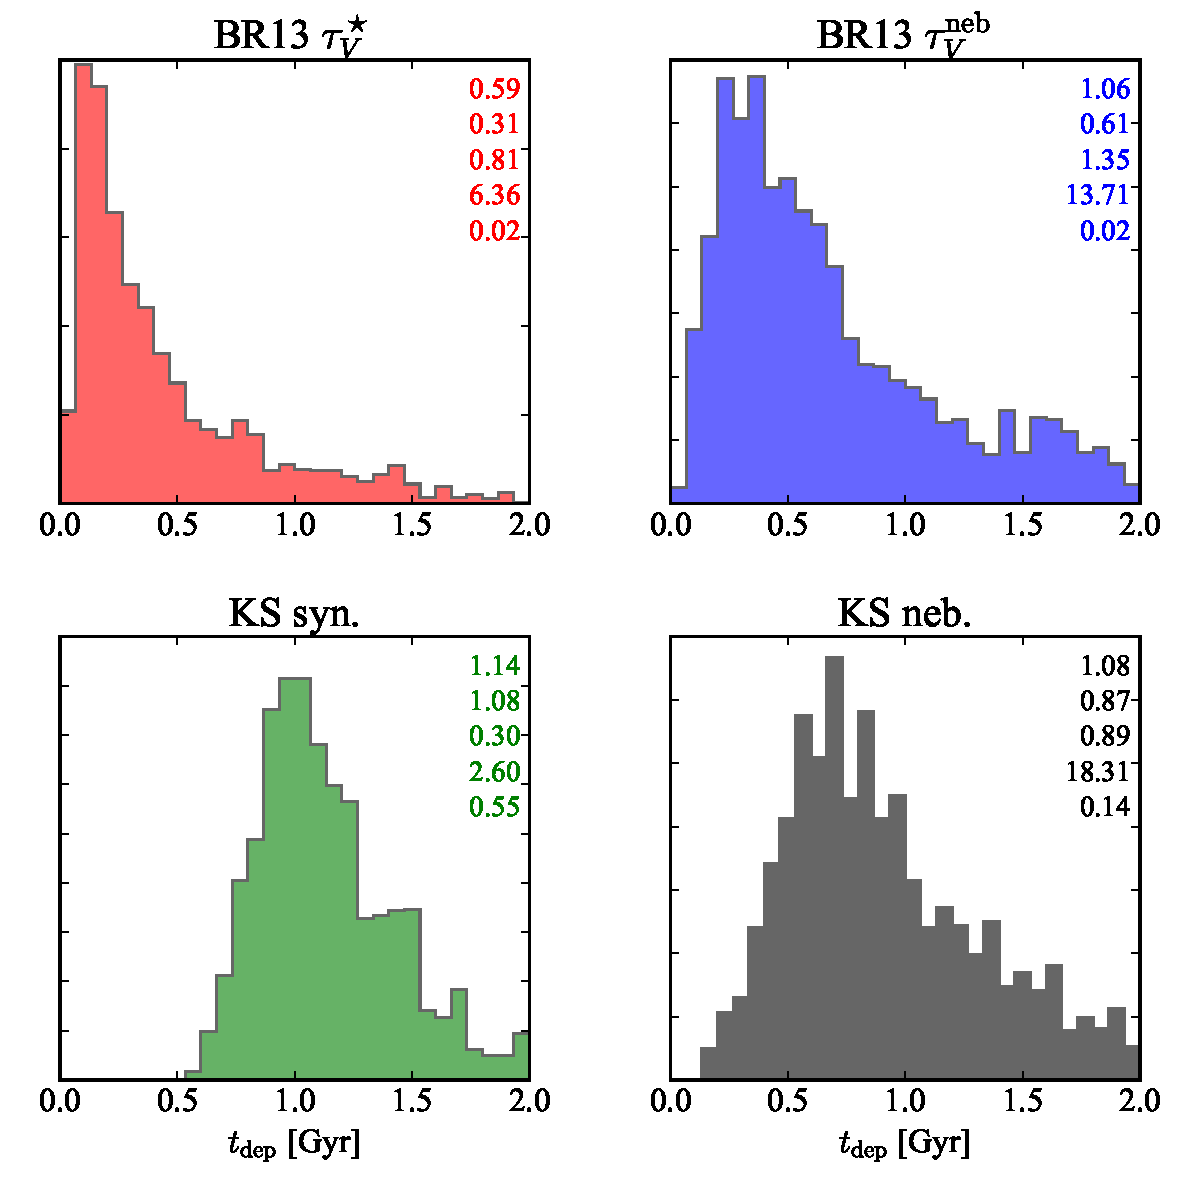
\includegraphics[width=0.99\textwidth]{figuras/histo_tdep.pdf}
	\caption[Tempo de depleção do gás]
	{Histogramas de $t_{\mathrm{dep}}$ para $\SigmaGas$ calculado como na Fig. \ref{fig:propsGasR}.
As cores e valores no canto superior direito de cada painel seguem o mesmo padrão da Fig. \ref{fig:histoGas}.}
	\label{fig:tdep}
\end{figure}

Também seria muito interessante fazer as mesmas análises que fizemos nos Caps. \ref{sec:difextin} e
\ref{sec:gasfrac} sobre as regiões \Hii do CALIFA mapeadas por \citet{Sanchez.etal.2012b}.
% \section{Eficiência e tempo de depleção do gás.}
% \label{sec:gasfrac:SFE}
% 
% Um outro tipo de abordagem é trabalhar com a eficiência da transformação de gás em estrelas,
% utilizando a relação:
% \begin{equation}
% 	\mathrm{SFE} = \frac{\Sigma_{\mathrm{SFR}}}{\Sigma_{\mathrm{gas}}} = \frac{1}{t_{\mathrm{dep}}},
% 	\label{eq:SFE}
% \end{equation}
% \noindent onde SFE vem de {\em star-formation efficiency} e $t_{\mathrm{dep}}$, que é o inverso da
% eficiência, é o tempo de depleção do gás, que nos dá uma ideia da escala de tempo em que a galáxia
% consome todo o gás com a taxa em que está formando estrelas.

%\ldots
%\chapter{Coeficiente de extinção como indicador de Gás}
%\label{sec:gas}
% Referências:
% - Brinchman
% - Guiderdoni & Rocca
% - procurar mais conversões dust to gas ou dust to stars
% - Referências para cada indicador
%\section{Indicadores de gás}
%\label{sec:synvsneb:proxies}
% Figuras:
% - ?? retiradas alguns papers para diferentes indicadores ??
%\section{Lei de Schimidt-Kennict}
%\label{sec:synvsneb:proxies}
% Figuras:
% - sample SK
% - our pseudo - SK
%\section{De poeira para gás}
%\label{sec:synvsneb:proxies}
% Figuras:
% - perfis radiais de SigmaGas e de fgas
% - real SK

% End of this chapter